% Dec 10 collation deck — Wang, Shaa, Privault, Guet (JCF)
% Case studies: synthetic constant-vol, synthetic Dupire, market data (placeholder)
% + IBP three-way diagnostic story
% Build: cd presentation && pdflatex dec10_collate.tex && pdflatex dec10_collate.tex
\documentclass[aspectratio=169,11pt]{beamer}

\usetheme{default}
\setbeamertemplate{navigation symbols}{}
\setbeamertemplate{footline}{}

\usepackage{booktabs}
\usepackage{amsmath,amssymb,amsfonts}
\usepackage{mathtools}
\usepackage{bm}
\usepackage{tikz}
\usetikzlibrary{shapes,arrows,positioning,calc}
\usepackage{xcolor}
\usepackage{graphicx}
\usepackage{hyperref}

\graphicspath{{figures/}{figures/dec10/}{figures/dec10_pdfs/}}

\definecolor{ntunavy}{RGB}{0,32,91}
\definecolor{ntudarkblue}{RGB}{0,20,60}
\definecolor{ntured}{RGB}{192,32,38}
\definecolor{ntugold}{RGB}{255,204,0}
\definecolor{ntulightblue}{RGB}{100,150,200}

\setbeamercolor{background canvas}{bg=ntunavy}
\setbeamercolor{normal text}{fg=white}
\setbeamercolor{frametitle}{fg=white}
\setbeamercolor{title}{fg=white}
\setbeamercolor{subtitle}{fg=ntugold}
\setbeamercolor{author}{fg=ntugold}
\setbeamercolor{institute}{fg=white}
\setbeamercolor{date}{fg=ntured}
\setbeamercolor{item}{fg=ntugold}
\setbeamercolor{structure}{fg=ntugold}
\setbeamercolor{block title}{fg=white,bg=ntured}
\setbeamercolor{block body}{fg=white,bg=ntunavy!70!black}

\setbeamerfont{title}{size=\Large,series=\bfseries}
\setbeamerfont{frametitle}{size=\large,series=\bfseries}
\setbeamertemplate{itemize item}{\scriptsize\raise1.5pt\hbox{\textbullet}}

\newcommand{\vect}[1]{\bm{#1}}

% NTU accent triangles on every slide
\setbeamertemplate{background}{
    \begin{tikzpicture}[remember picture,overlay]
        \shade[left color=ntunavy,right color=ntudarkblue,shading angle=-45]
            (current page.north west) rectangle (current page.south east);
        \fill[ntured]
            (current page.north west) --
            ([xshift=1.8cm]current page.north west) --
            ([yshift=-2.7cm]current page.north west) -- cycle;
        \fill[ntured!85!black]
            ([yshift=-2.2cm]current page.north west) --
            ([xshift=1.4cm,yshift=-2.2cm]current page.north west) --
            ([yshift=-4.0cm]current page.north west) -- cycle;
    \end{tikzpicture}
}

% Title page template (matching main.tex)
\defbeamertemplate*{title page}{ntu}[1][]
{
    \begin{tikzpicture}[remember picture,overlay]
        \shade[left color=ntunavy,right color=ntudarkblue!90!ntunavy,shading angle=-30]
            (current page.north west) rectangle (current page.south east);
        \fill[ntured]
            (current page.north west) --
            ([xshift=2.2cm]current page.north west) --
            ([yshift=-3.3cm]current page.north west) -- cycle;
        \IfFileExists{ntu_logo.jpg}{
            \node[anchor=north west] at ([xshift=0.5cm,yshift=-0.4cm]current page.north west) {
                
\includegraphics[height=1.2cm]{ntu_logo.jpg}
            };
        }{}
        \node[anchor=north west, text width=10cm, font=\fontsize{11}{13}\selectfont\bfseries]
            at ([xshift=2.8cm,yshift=-2.3cm]current page.north west) {
            \textcolor{ntugold}{Dupire PINN / PDF validation}
        };
        \node[anchor=north west, text width=10.5cm]
            at ([xshift=2.8cm,yshift=-3.0cm]current page.north west) {
            {\fontsize{20}{24}\selectfont\bfseries\color{white}\inserttitle}
        };
        \node[anchor=north west, text width=10cm, font=\fontsize{12}{14}\selectfont\bfseries]
            at ([xshift=2.8cm,yshift=-5.4cm]current page.north west) {
            \textcolor{ntugold}{\insertauthor}
        };
        \node[anchor=north west, text width=10cm, font=\fontsize{8}{10}\selectfont]
            at ([xshift=2.8cm,yshift=-6.0cm]current page.north west) {
            \textcolor{white}{\insertinstitute}
        };
        \node[anchor=north west, font=\fontsize{10}{12}\selectfont\bfseries]
            at ([xshift=2.8cm,yshift=-7.2cm]current page.north west) {
            \textcolor{ntured}{\insertdate}
        };
    \end{tikzpicture}
}

\setbeamertemplate{frametitle}{
    \vspace{0.3cm}
    \hspace{2.5cm}{\usebeamerfont{frametitle}\insertframetitle}
    \vspace{0.1cm}
}

\title{PDF validation \& IBP diagnostic:\\three case studies}
\subtitle{Wang Z., Shaa A., Privault N., Guet C.}
\author{Ameir Shaa}
\date{December 2025 / May 2026}
\institute{JCF manuscript --- LocalVolatility PINN pipeline}

%% ============================================================
\begin{document}
\maketitle

%% ---- OUTLINE -----------------------------------------------
\begin{frame}{Outline}
    \tableofcontents
\end{frame}

%% ============================================================
\section{Overview}
%% ============================================================

\begin{frame}{Paper overview}
    \textbf{Wang, Shaa, Privault, Guet} --- JCF manuscript
    \vspace{0.3cm}

    Two physics-informed neural networks calibrate Dupire local volatility:
    \begin{itemize}
        \item \texttt{NN\_phi}: ansatz $\tilde\varphi(T,K) = 1 - e^{-\mathrm{NN}_\varphi(T,K)}$ encodes call-price positivity and $K\to\infty$ decay
        \item \texttt{NN\_eta}: local variance $\tilde\eta(T,K) = \sigma^2(T,K)$ fed directly into Dupire PDE
    \end{itemize}

    \vspace{0.3cm}
    \textbf{Three case studies:}
    \begin{enumerate}
        \item Synthetic constant volatility $\sigma = 1$
        \item Synthetic non-constant Dupire volatility (manuscript formula, \S4.1)
        \item Market data --- DAX Aug 2001 / SPX May 2019
    \end{enumerate}
    \vspace{0.25cm}
    \textbf{Validation:} PDF analysis (MC histogram vs NN density) + IBP three-way mean diagnostic
\end{frame}

%% ============================================================
\section{Synthetic: constant volatility ($\sigma=1$)}
%% ============================================================

\begin{frame}{Case 1 setup: constant volatility $\sigma = 1$}
    \begin{columns}[T]
        \begin{column}{0.55\textwidth}
            \textbf{Model:} $dS_t = r S_t \, dt + S_t \, dW_t$ \quad ($r=0.02$, $S_0=1000$)

            \vspace{0.25cm}
            \textbf{Training data:} synthetic option prices from Black--Scholes closed form

            \vspace{0.25cm}
            \textbf{Strike range:} $K \in [500, 3000]$

            \vspace{0.25cm}
            \textbf{Maturities:} $T \in \{0.5, 1.0, 1.5\}$

            \vspace{0.25cm}
            \textbf{Benchmark:} analytical BS density (log-normal)
        \end{column}
        \begin{column}{0.42\textwidth}
            \textbf{Key quantities:}
            \begin{itemize}
                \item Forward $S_0 e^{rT}$
                \item NN density $\partial^2 C_{\mathrm{NN}} / \partial K^2$ vs MC histogram
                \item IBP mean $M_1 = e^{rT}\int K\,\partial^2 C/\partial K^2\,dK$
                \item $M_2 = e^{rT} C_{\mathrm{NN}}(0,T)$
                \item $M_3 = \mathbb{E}[S_T]$ from MC
            \end{itemize}
        \end{column}
    \end{columns}
\end{frame}

\begin{frame}{Case 1: constant vol --- PDF analysis (pretrained model)}
    \begin{center}
        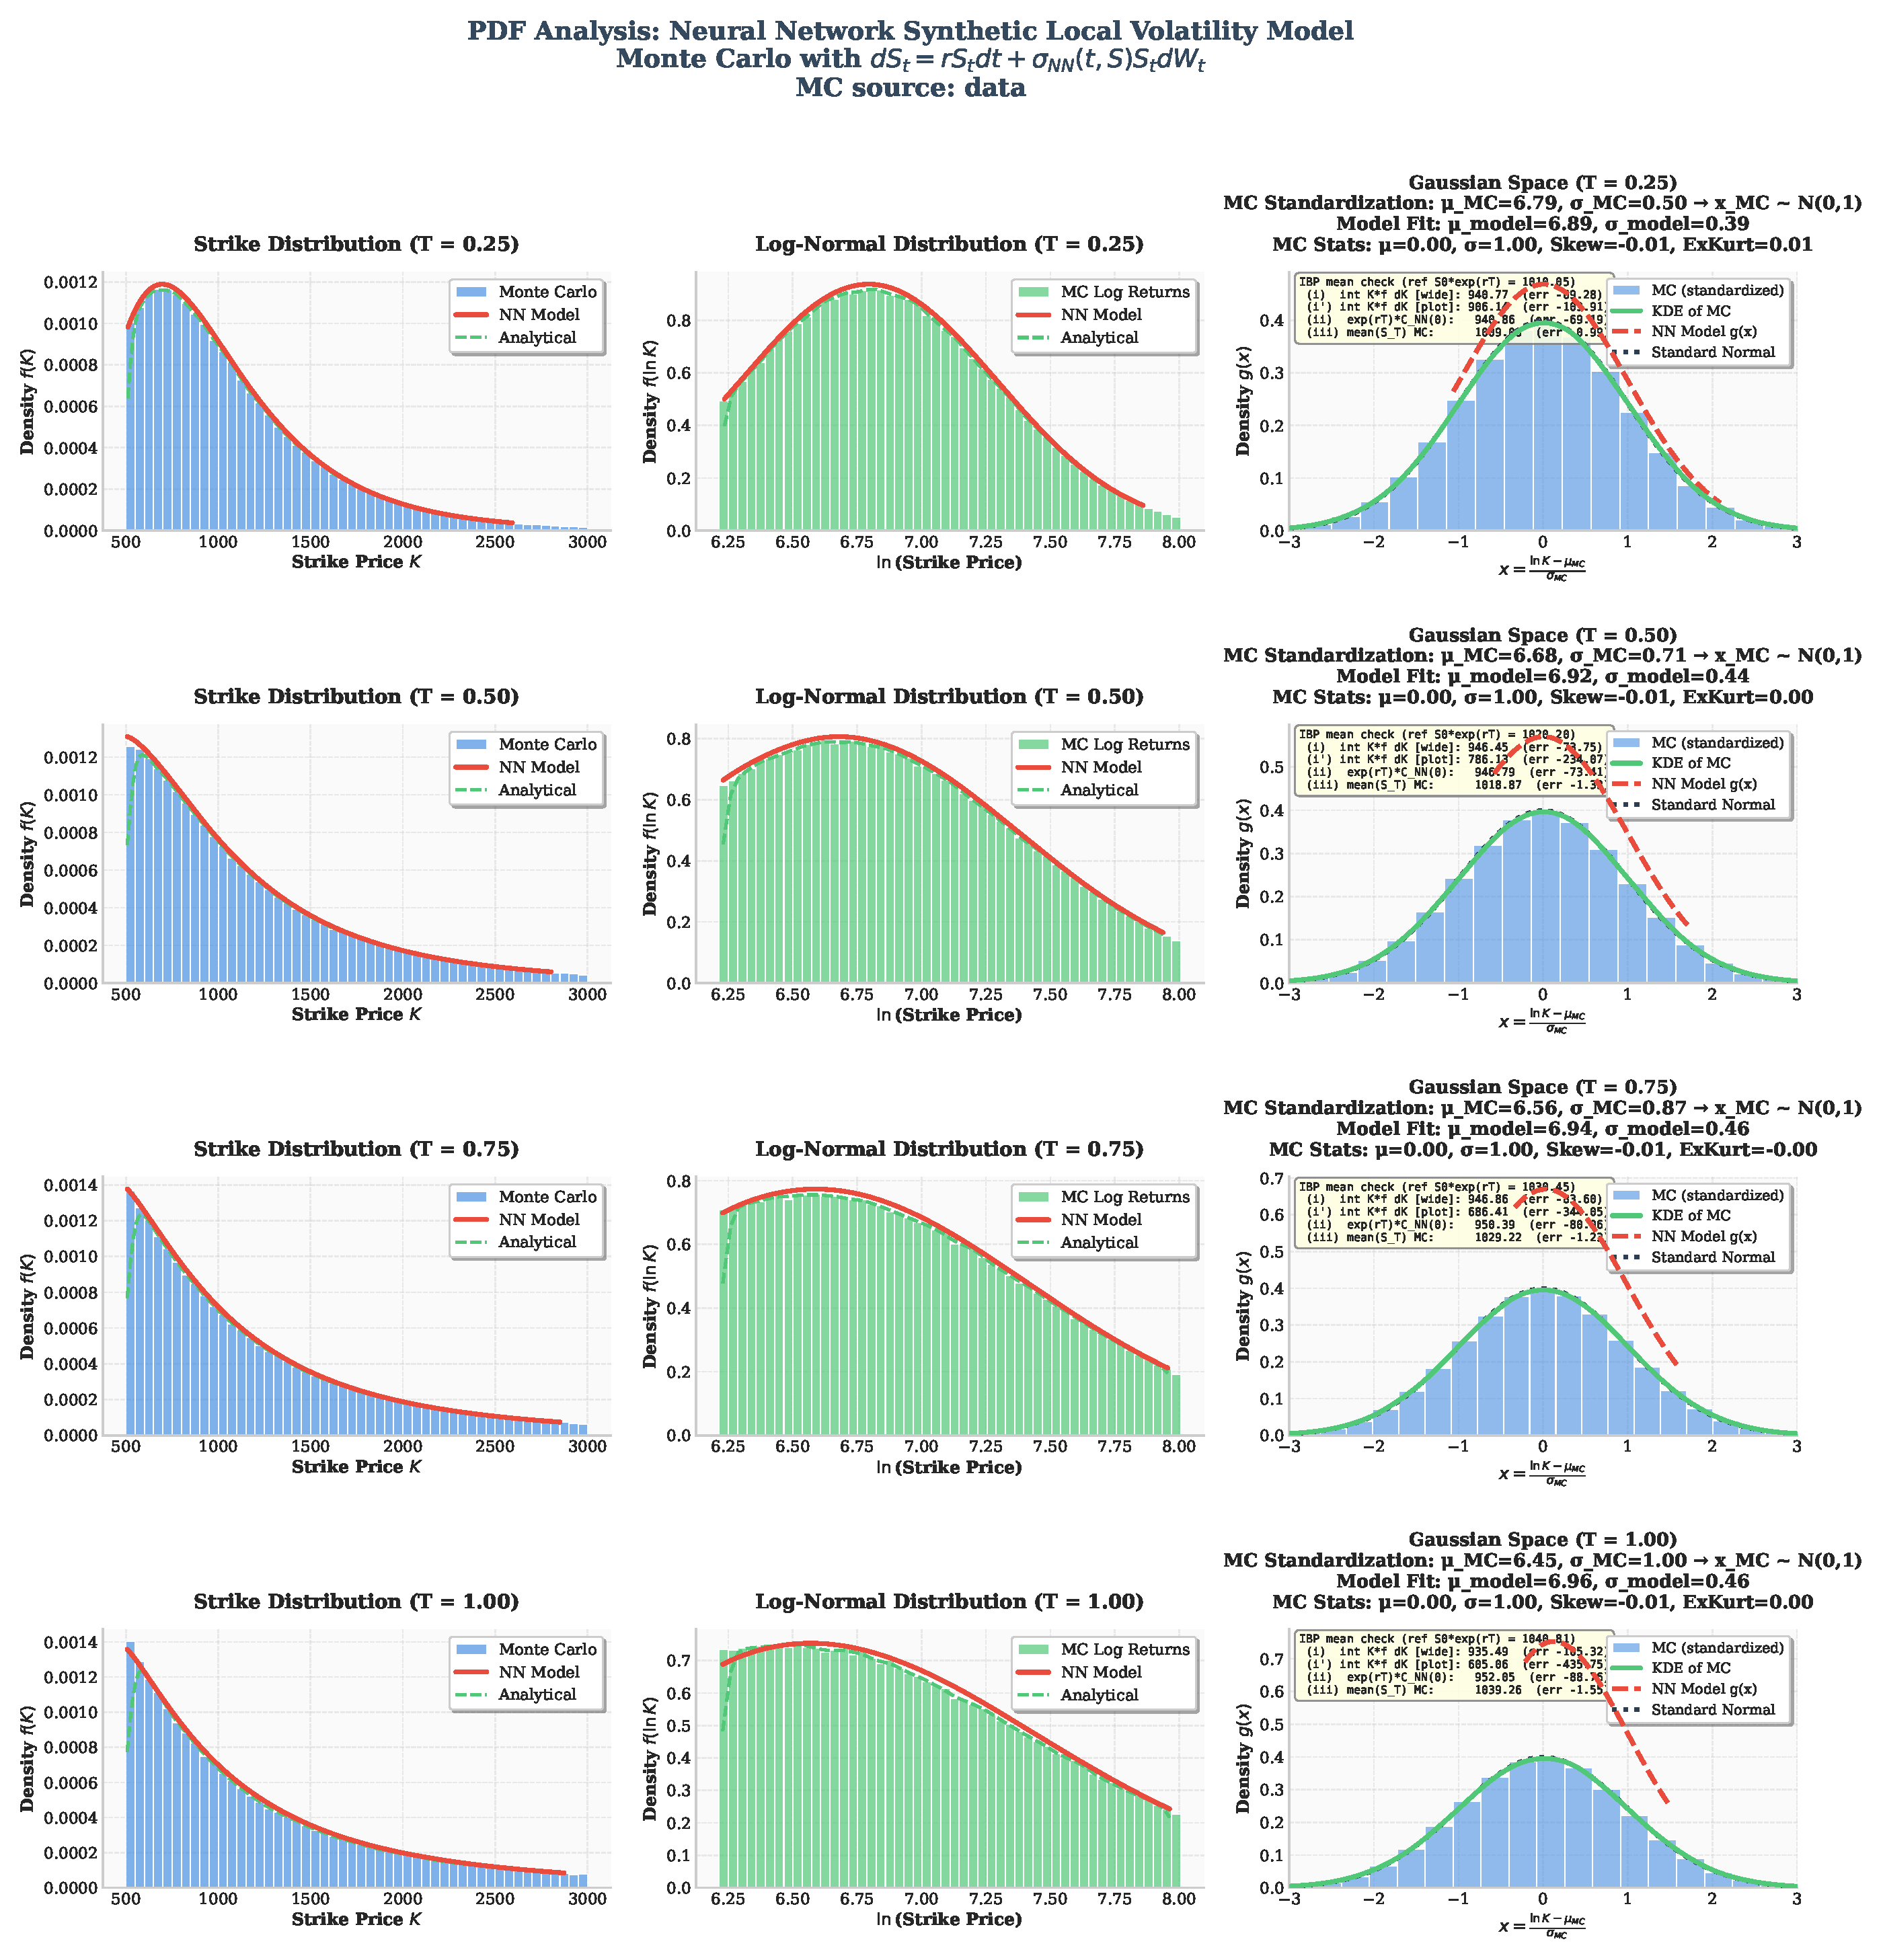
\includegraphics[width=0.98\linewidth,height=0.80\textheight,keepaspectratio]{syn_const_pretrained.pdf}
    \end{center}
    \vspace{-0.1cm}
    {\footnotesize \textbf{MC source: data.}
    Strike-space (left), log-strike (centre), Gaussian-standardized (right).
    IBP box (upper right of each Gaussian panel) shows $M_1, M_2 \approx 7\%$ below
    forward at every $T$ --- NN$_\varphi$ undershoots near $K=0$.}
\end{frame}

\begin{frame}{Case 1: constant vol --- PDF analysis (repriced)}
    \begin{center}
        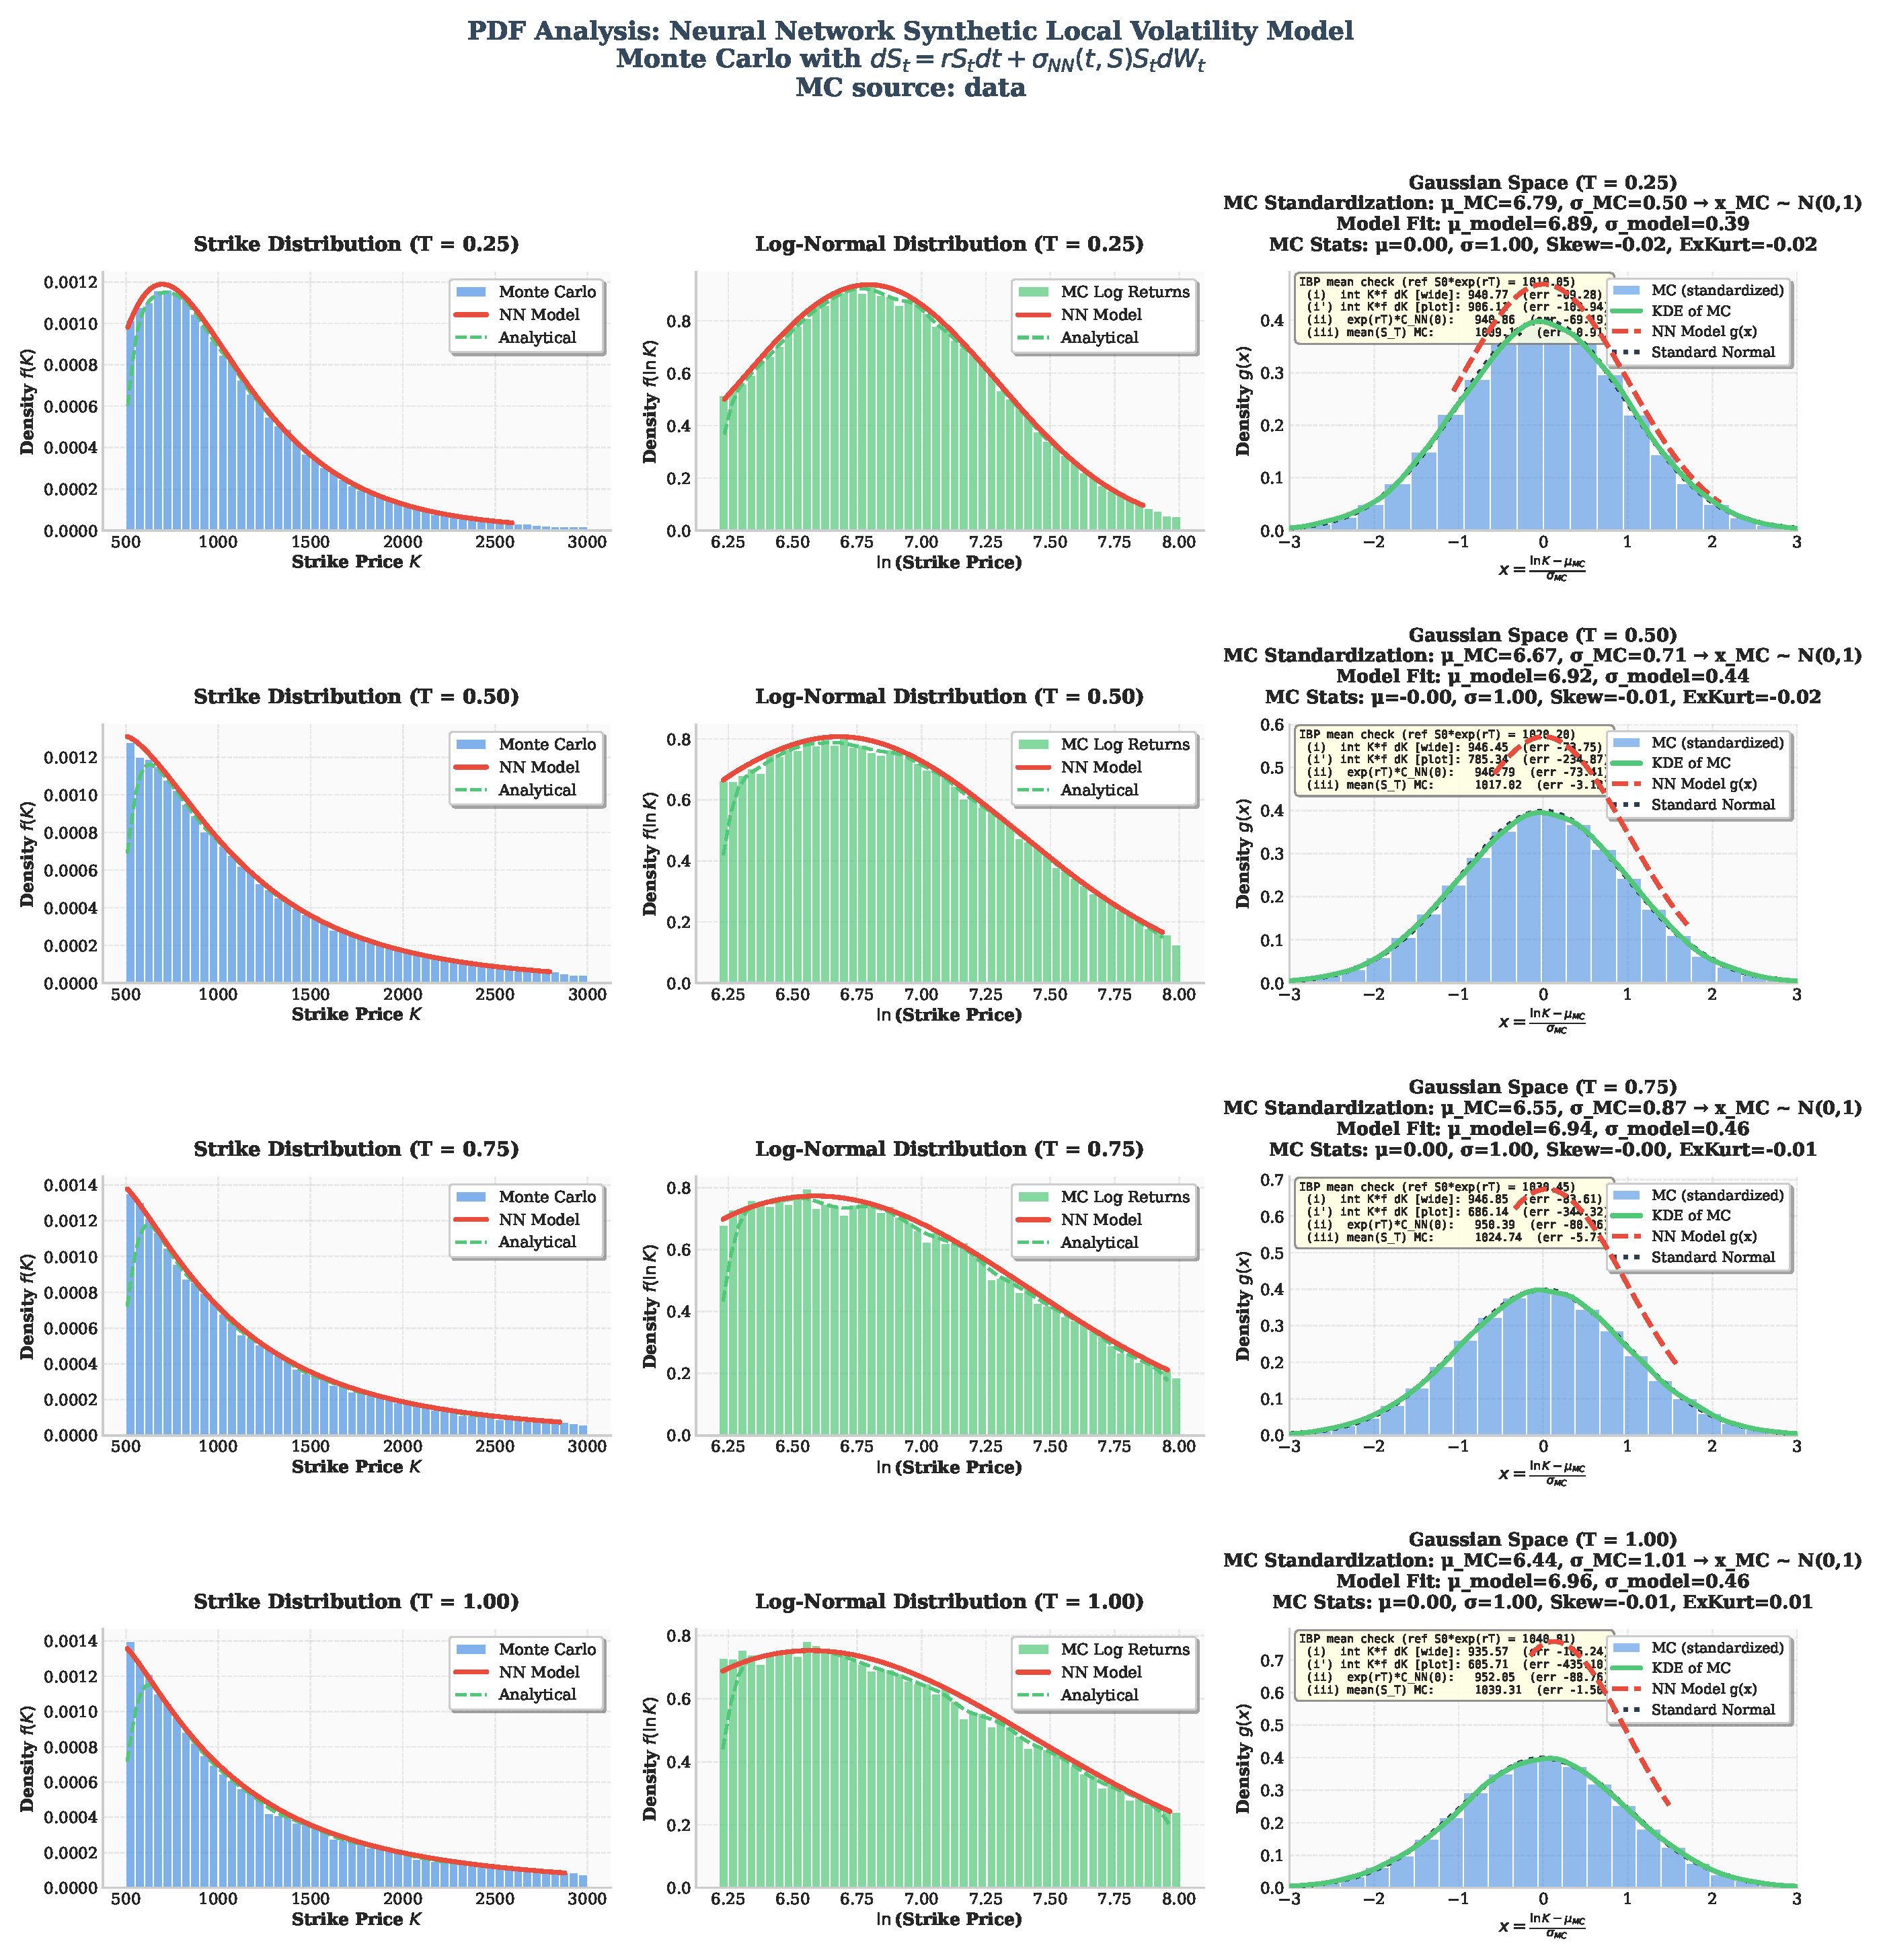
\includegraphics[width=0.98\linewidth,height=0.80\textheight,keepaspectratio]{syn_const_repriced.pdf}
    \end{center}
    \vspace{-0.1cm}
    {\footnotesize \textbf{MC source: repriced.}
    Same model; MC paths generated with the NN-implied $\sigma(t,S)$.
    $M_3$ now tracks the NN-implied forward --- cross-validates NN$_\eta$ MC.}
\end{frame}

\begin{frame}{Case 1: constant vol $\sigma=1$ --- PDF analysis (Dec 9 2025)}
    \begin{center}
        \includegraphics[width=0.92\linewidth]{figures/dec10_pdfs/syn_const_sigma.png}
    \end{center}
    \vspace{-0.1cm}
    {\footnotesize \textbf{Dec 9 2025 run.}
    Synthetic constant volatility $\sigma=1$, $K\in[500,3000]$, $T\in\{0.25,0.50,0.75,1.00\}$.
    $\sigma_{\mathrm{MC}}$ tracks $\sigma_{\mathrm{truth}}\cdot\sqrt{T}$ exactly ($\approx0.50,0.71,0.87,1.00$).
    NN model is essentially indistinguishable from MC and analytical log-normal density.}
\end{frame}

\begin{frame}{Case 1: IBP mean diagnostics (pretrained model)}
    \footnotesize
    \setlength{\tabcolsep}{4pt}
    \centering
    \begin{tabular}{r r r r r r r r r r}
        \toprule
        $T$ & $M_{\mathrm{ref}}$ & $M_1$ & \%err & $M_2$ & \%err & $M_3$ & \%err & $\Delta M_{12}$\% & $\Delta M_{13}$\% \\
        \midrule
        0.5 & 1020.20 &  948.87 & $-6.99$ &  948.93 & $-6.99$ & 1018.25 & $-0.19$ & 0.006 & 6.814 \\
        1.0 & 1040.81 &  967.66 & $-7.03$ &  967.74 & $-7.02$ & 1038.19 & $-0.25$ & 0.009 & 6.794 \\
        1.5 & 1061.84 &  982.49 & $-7.47$ &  982.95 & $-7.43$ & 1054.36 & $-0.70$ & 0.047 & 6.816 \\
        \bottomrule
    \end{tabular}

    \vspace{0.5em}
    \scriptsize
    \begin{itemize}
        \item $M_1 \equiv M_2$ to $<\!0.05\%$ at all $T$ $\Rightarrow$ IBP identity holds exactly in the code.
        \item $M_3$ within $0.7\%$ of forward $\Rightarrow$ NN$_\eta$ MC well-calibrated.
        \item $M_1, M_2 \approx 7\%$ below forward $\Rightarrow$ NN$_\varphi$ undershoots at $K \to 0$.
    \end{itemize}

\end{frame}

%% ============================================================
\section{Synthetic: manuscript Dupire volatility}
%% ============================================================

\begin{frame}{Case 2 setup: non-constant Dupire volatility}
    \textbf{Manuscript formula} (\S4.1):
    \[
        \sigma(x, t) = 0.3 + y\, e^{-y},
        \qquad y = (t + 0.1)\sqrt{x + 0.1}
    \]
    where $x = S_t$, producing a non-trivial $\sigma^2(K, T)$ surface.

    \vspace{0.3cm}
    \begin{columns}[T]
        \begin{column}{0.55\textwidth}
            \begin{itemize}
                \item $S_0 = 1000$, $r = 0.02$
                \item Strike range $K \in [500, 3000]$
                \item Maturities $T \in \{0.25, 0.50, 0.75, 1.00\}$
                \item Training data generated from the exact formula (not market quotes)
            \end{itemize}
        \end{column}
        \begin{column}{0.42\textwidth}
            \begin{itemize}
                \item Benchmark: analytical density from exact $\sigma(x,t)$
                \item NN must recover non-flat $\sigma^2(K,T)$ surface from prices alone
                \item IBP diagnostics: same three-way check as Case 1
            \end{itemize}
        \end{column}
    \end{columns}
\end{frame}

\begin{frame}{Case 2: Dupire vol --- PDF analysis (pretrained model)}
    \begin{center}
        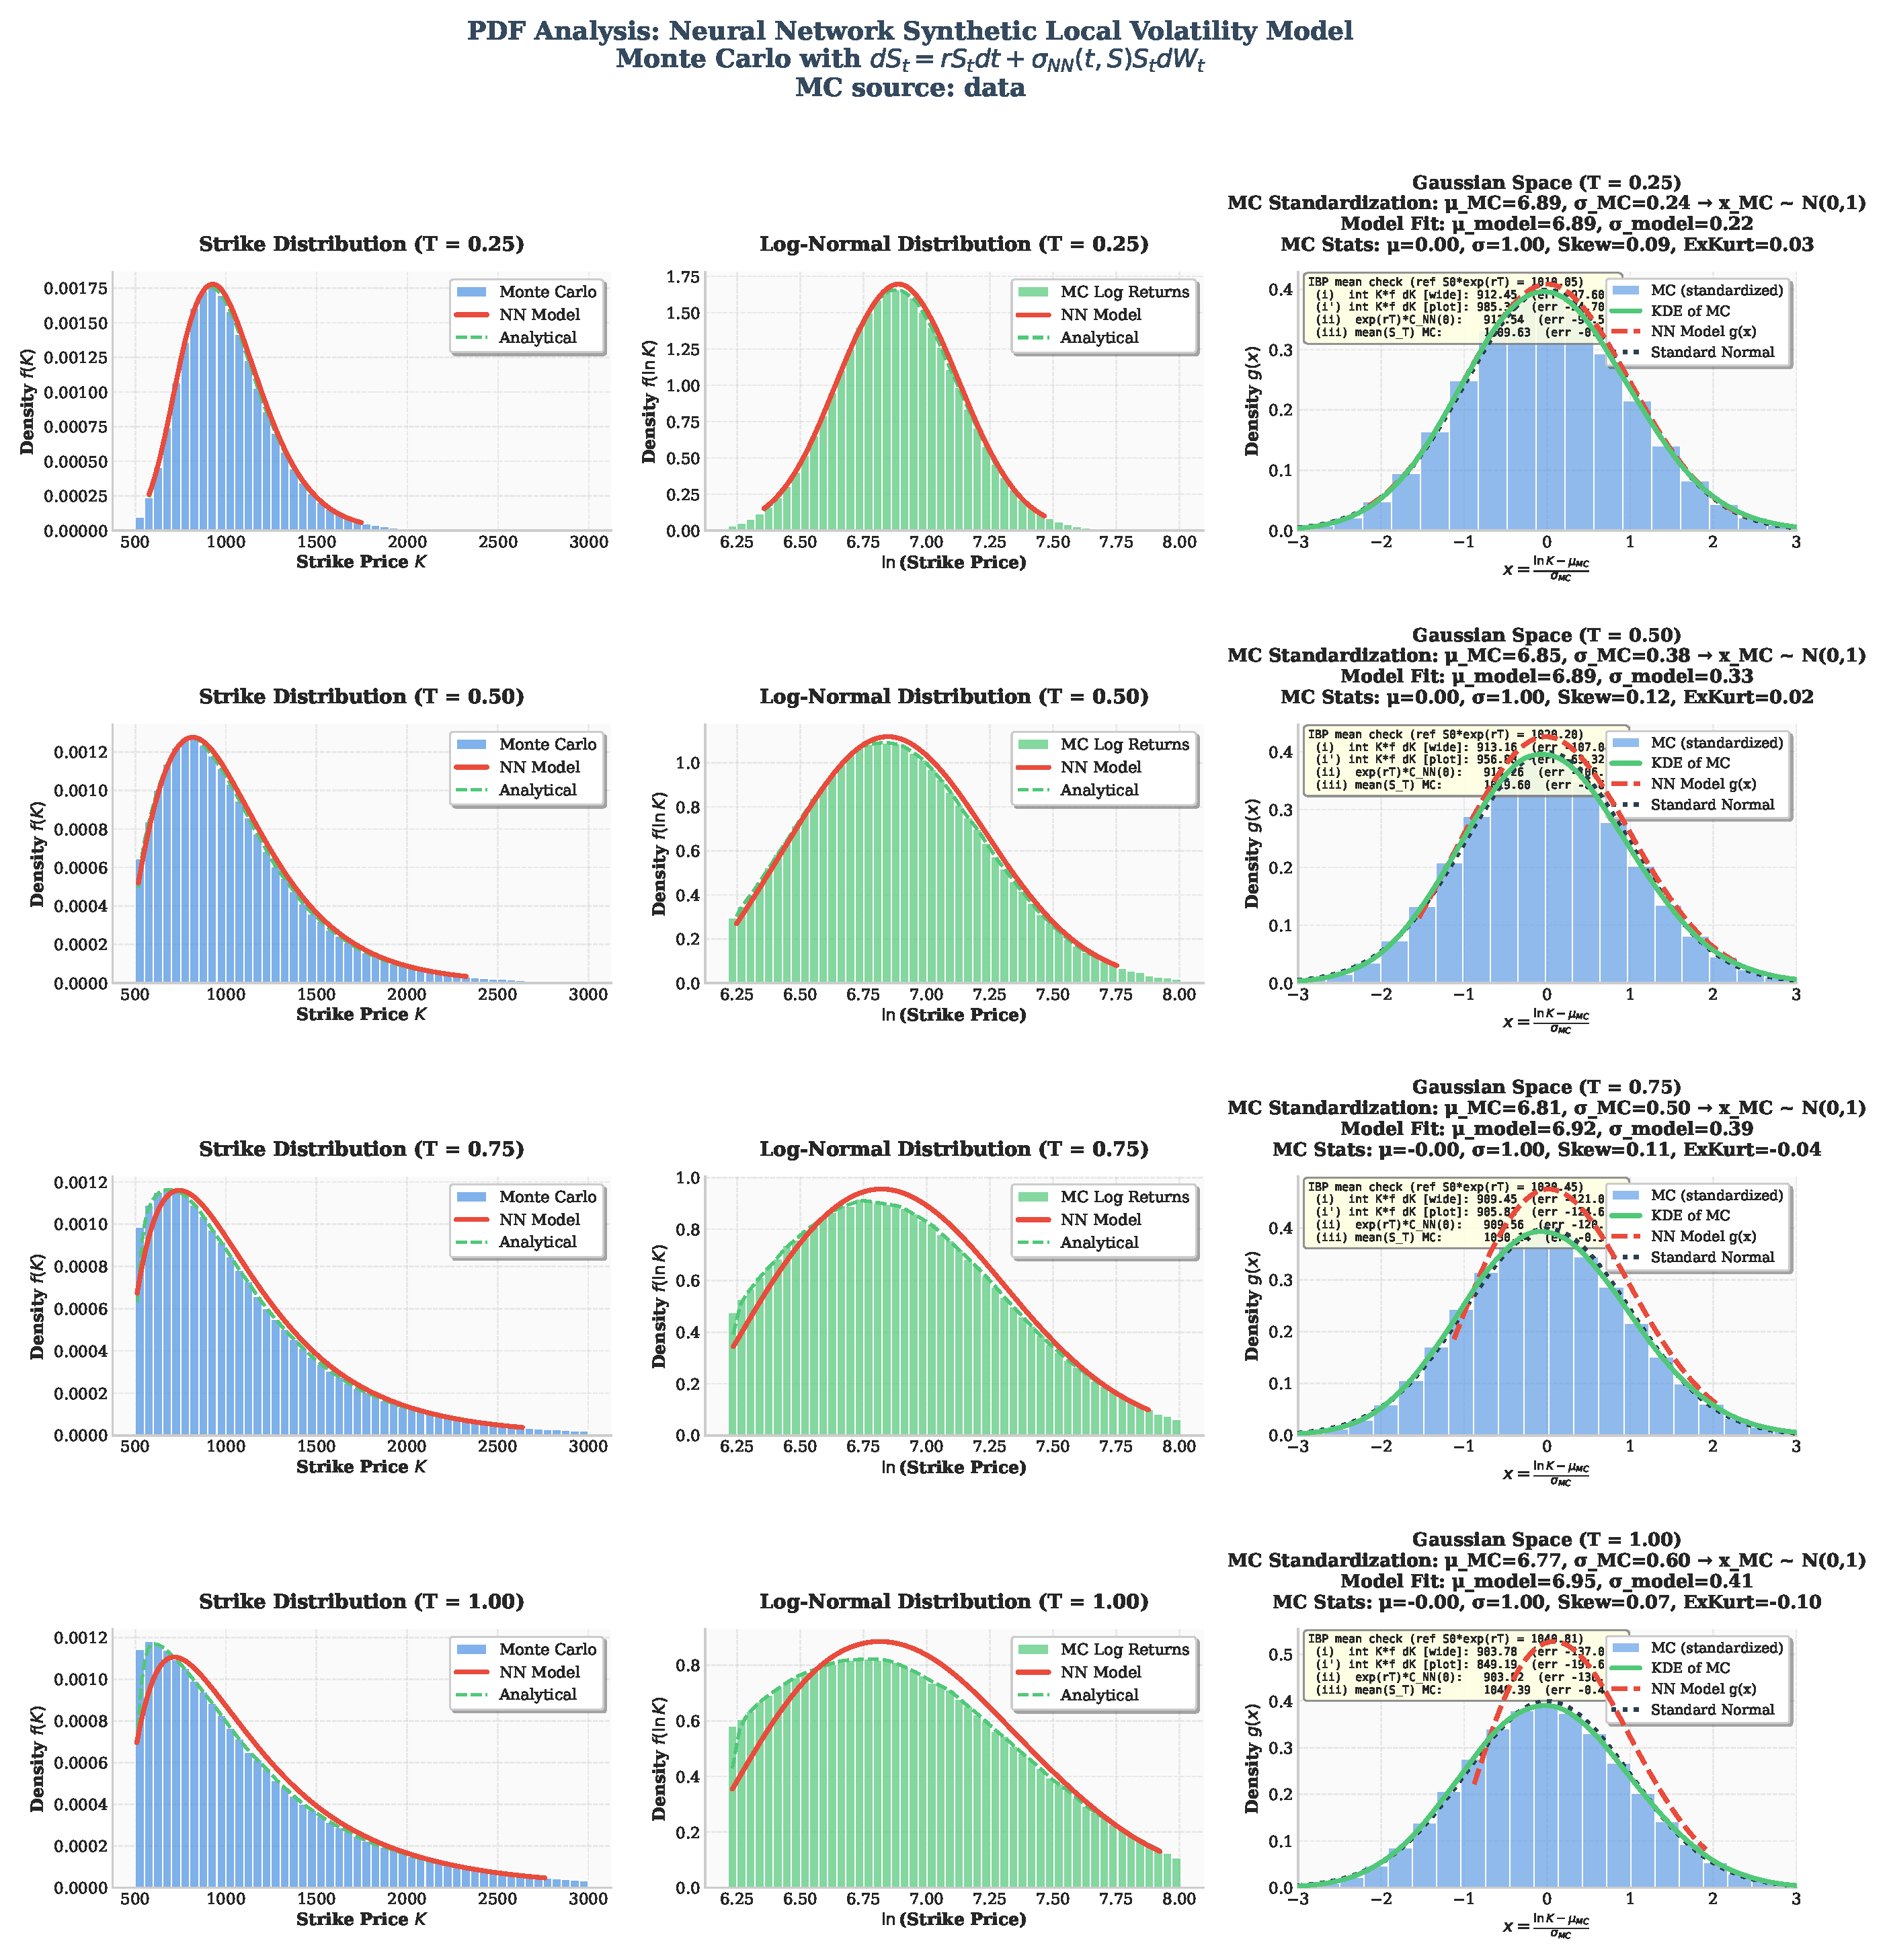
\includegraphics[width=0.98\linewidth,height=0.80\textheight,keepaspectratio]{syn_nonconst_pretrained.pdf}
    \end{center}
    \vspace{-0.1cm}
    {\footnotesize \textbf{MC source: data.}
    Non-constant $\sigma(x,t)$ produces a skewed, non-log-normal density (visible in log-strike panel).
    NN (red) tracks the analytical (dashed) and MC histogram closely at all four maturities.
    IBP box shows $M_1, M_2 \approx 7$--$14\%$ below forward at $T \ge 0.5$.}
\end{frame}

\begin{frame}{Case 2: Dupire vol --- PDF analysis (repriced)}
    \begin{center}
        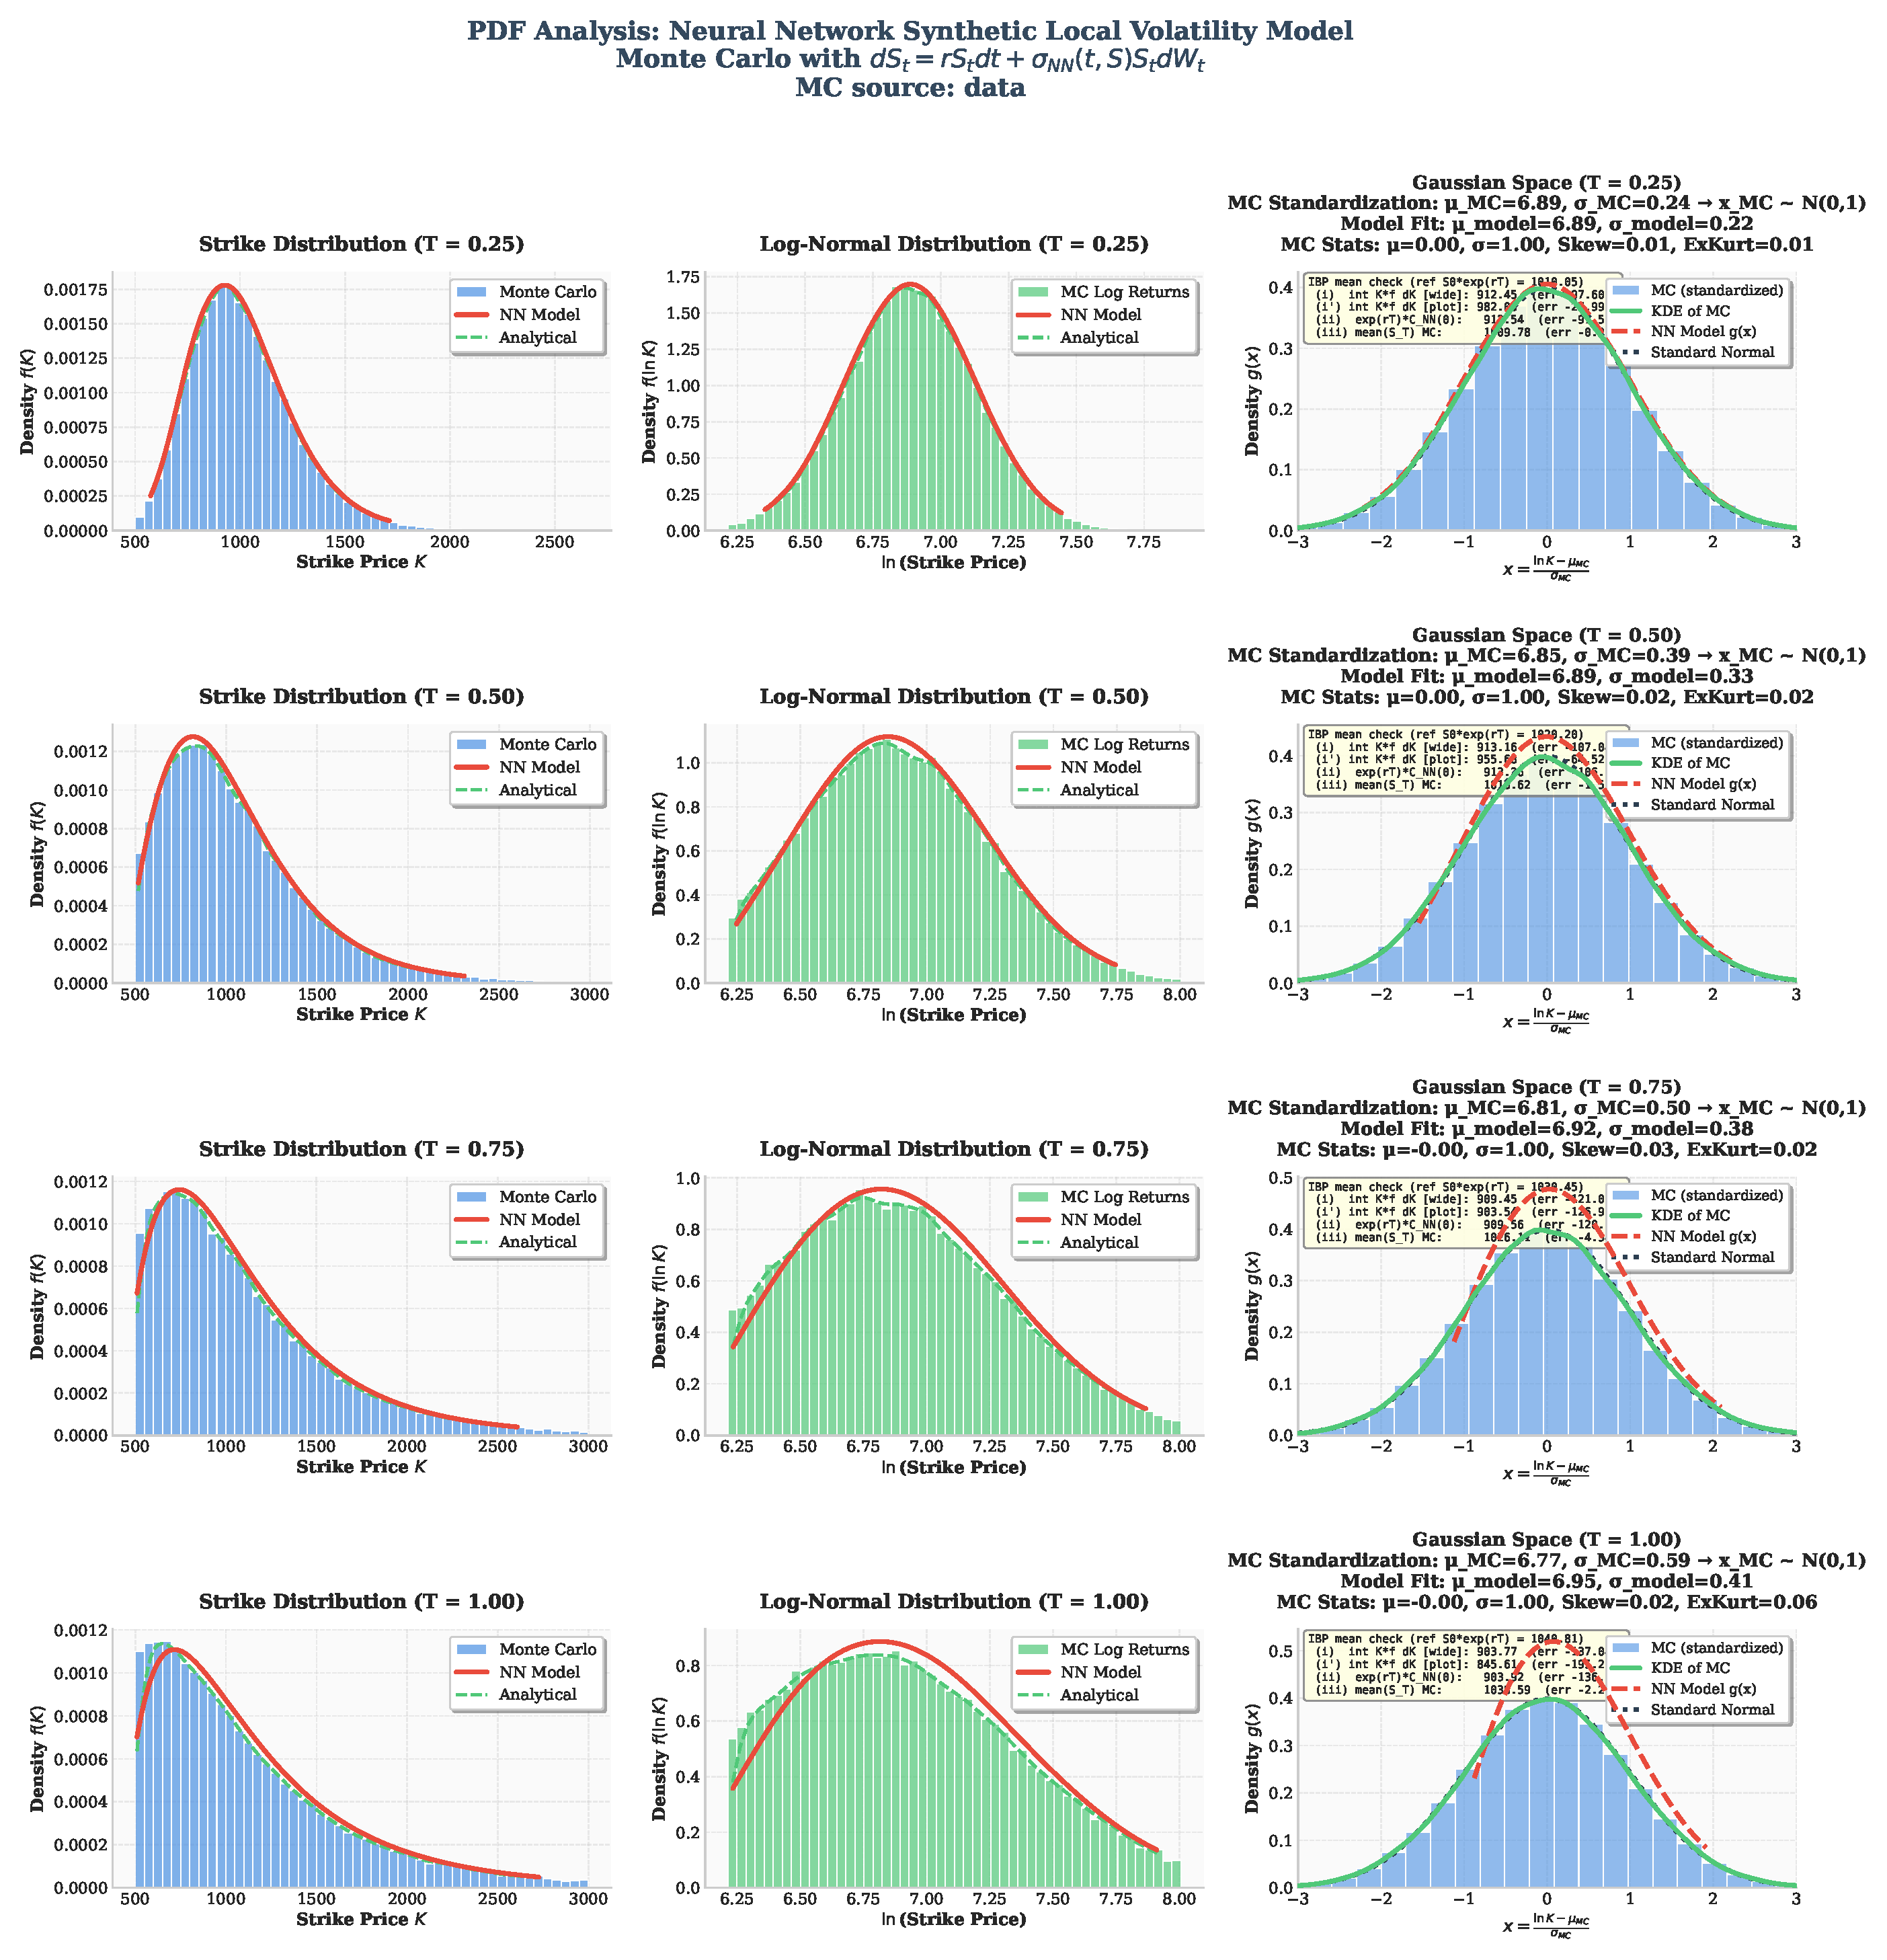
\includegraphics[width=0.98\linewidth,height=0.80\textheight,keepaspectratio]{syn_nonconst_repriced.pdf}
    \end{center}
    \vspace{-0.1cm}
    {\footnotesize \textbf{MC source: repriced.}
    MC paths driven by NN-implied $\sigma(t,S)$. Shape match in Gaussian space confirms
    NN$_\eta$ recovers the non-flat surface; IBP deficit persists (same K=0 undershoot).}
\end{frame}

\begin{frame}{Case 2: Dupire non-constant vol --- PDF analysis (Dec 7 2025)}
    \begin{center}
        \includegraphics[width=0.92\linewidth]{figures/dec10_pdfs/syn_dupire_nonconst.png}
    \end{center}
    \vspace{-0.1cm}
    {\footnotesize \textbf{Dec 7 2025 run.}
    Synthetic Dupire: $\sigma(x,t)=0.3+ye^{-y}$, $y=(t+0.1)\sqrt{x+0.1}$;
    $K\in[500,3000]$, $T\in\{0.25,0.50,0.75,1.00\}$.
    $\sigma_{\mathrm{MC}}\approx0.24,0.38,0.50,0.59$ across maturities.
    NN model, MC, and analytical KDE-of-MC agree closely across all four maturities.}
\end{frame}

%% ============================================================
\section{Market data}
%% ============================================================

\begin{frame}{Case 3: Market data --- context}
    \textbf{DAX Aug 7--9 2001}: European index options, 3-day window.

    \vspace{0.2cm}
    \begin{itemize}
        \item $K \in [4000, 9000]$, $T \in \{0.12, 0.20, 0.37, 0.60, 0.87\}$
        \item NN trained on DAX market quotes; MC driven by NN-implied $\sigma(t,S)$
        \item $\mu_{\mathrm{MC}} \approx 8.64\text{--}8.66$ (in $\ln K$ space)
        \item NN model deviates noticeably from MC/analytical in $K$-space (visible panel 1)
        \item Gaussian-space MC tracks $\mathcal{N}(0,1)$; NN $g(x)$ deviates --- K=0 boundary fingerprint
    \end{itemize}

    \vspace{0.3cm}
    {\small\color{ntugold}
        Provisional day-to-file assignment inferred from chronological filename order.
        \textbf{Confirm via raw data} if day ordering matters for interpretation.}
\end{frame}

\begin{frame}{Case 3: DAX Aug 7, 2001 --- PDF analysis}
    \begin{center}
        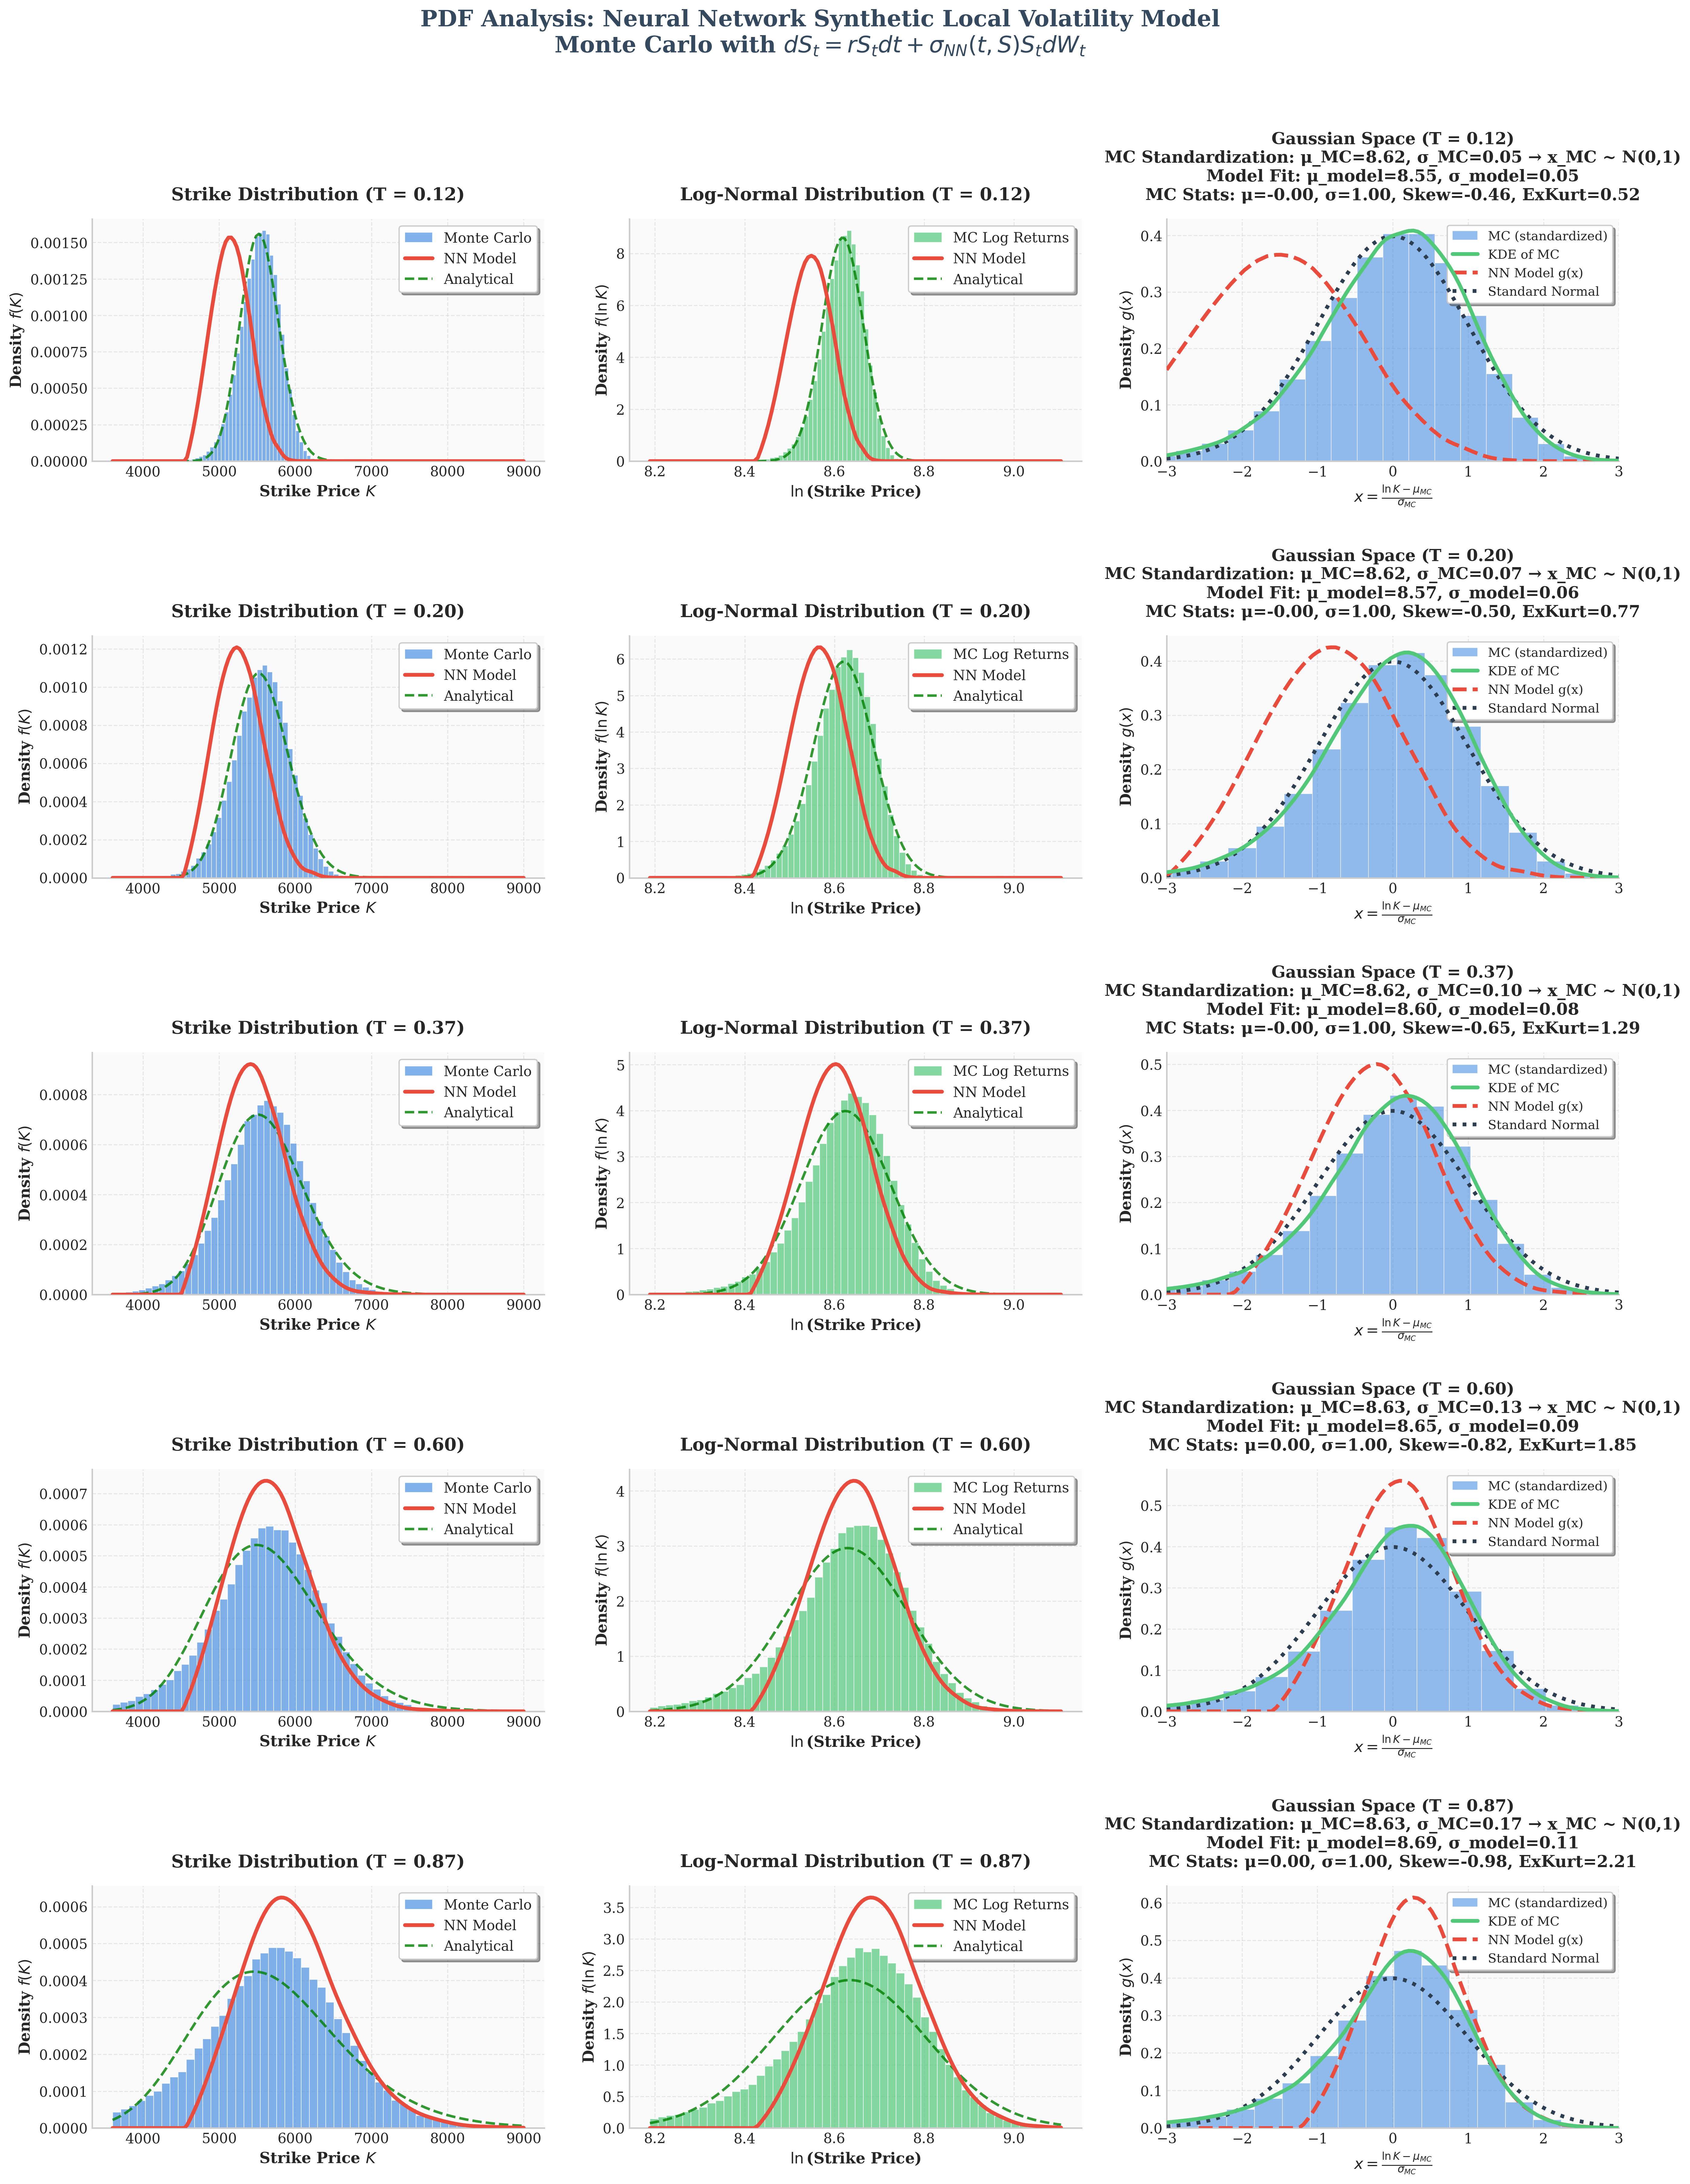
\includegraphics[width=0.92\linewidth]{figures/dec10_pdfs/dax_day1_aug7.png}
    \end{center}
    \vspace{-0.1cm}
    {\footnotesize \textbf{DAX Aug 7 2001} (provisional day assignment --- confirm via raw data).
    $K\in[4000,9000]$, $T\in\{0.12,0.20,0.37,0.60,0.87\}$; $\mu_{\mathrm{MC}}=8.64$ ($\ln K$).
    Panel 1 (K-space): NN-vs-MC deviation visible; Gaussian panel: MC $\approx\mathcal{N}(0,1)$, NN $g(x)$ deviates --- K=0-boundary fingerprint (see IBP section).}
\end{frame}

\begin{frame}{Case 3: DAX Aug 8, 2001 --- PDF analysis}
    \begin{center}
        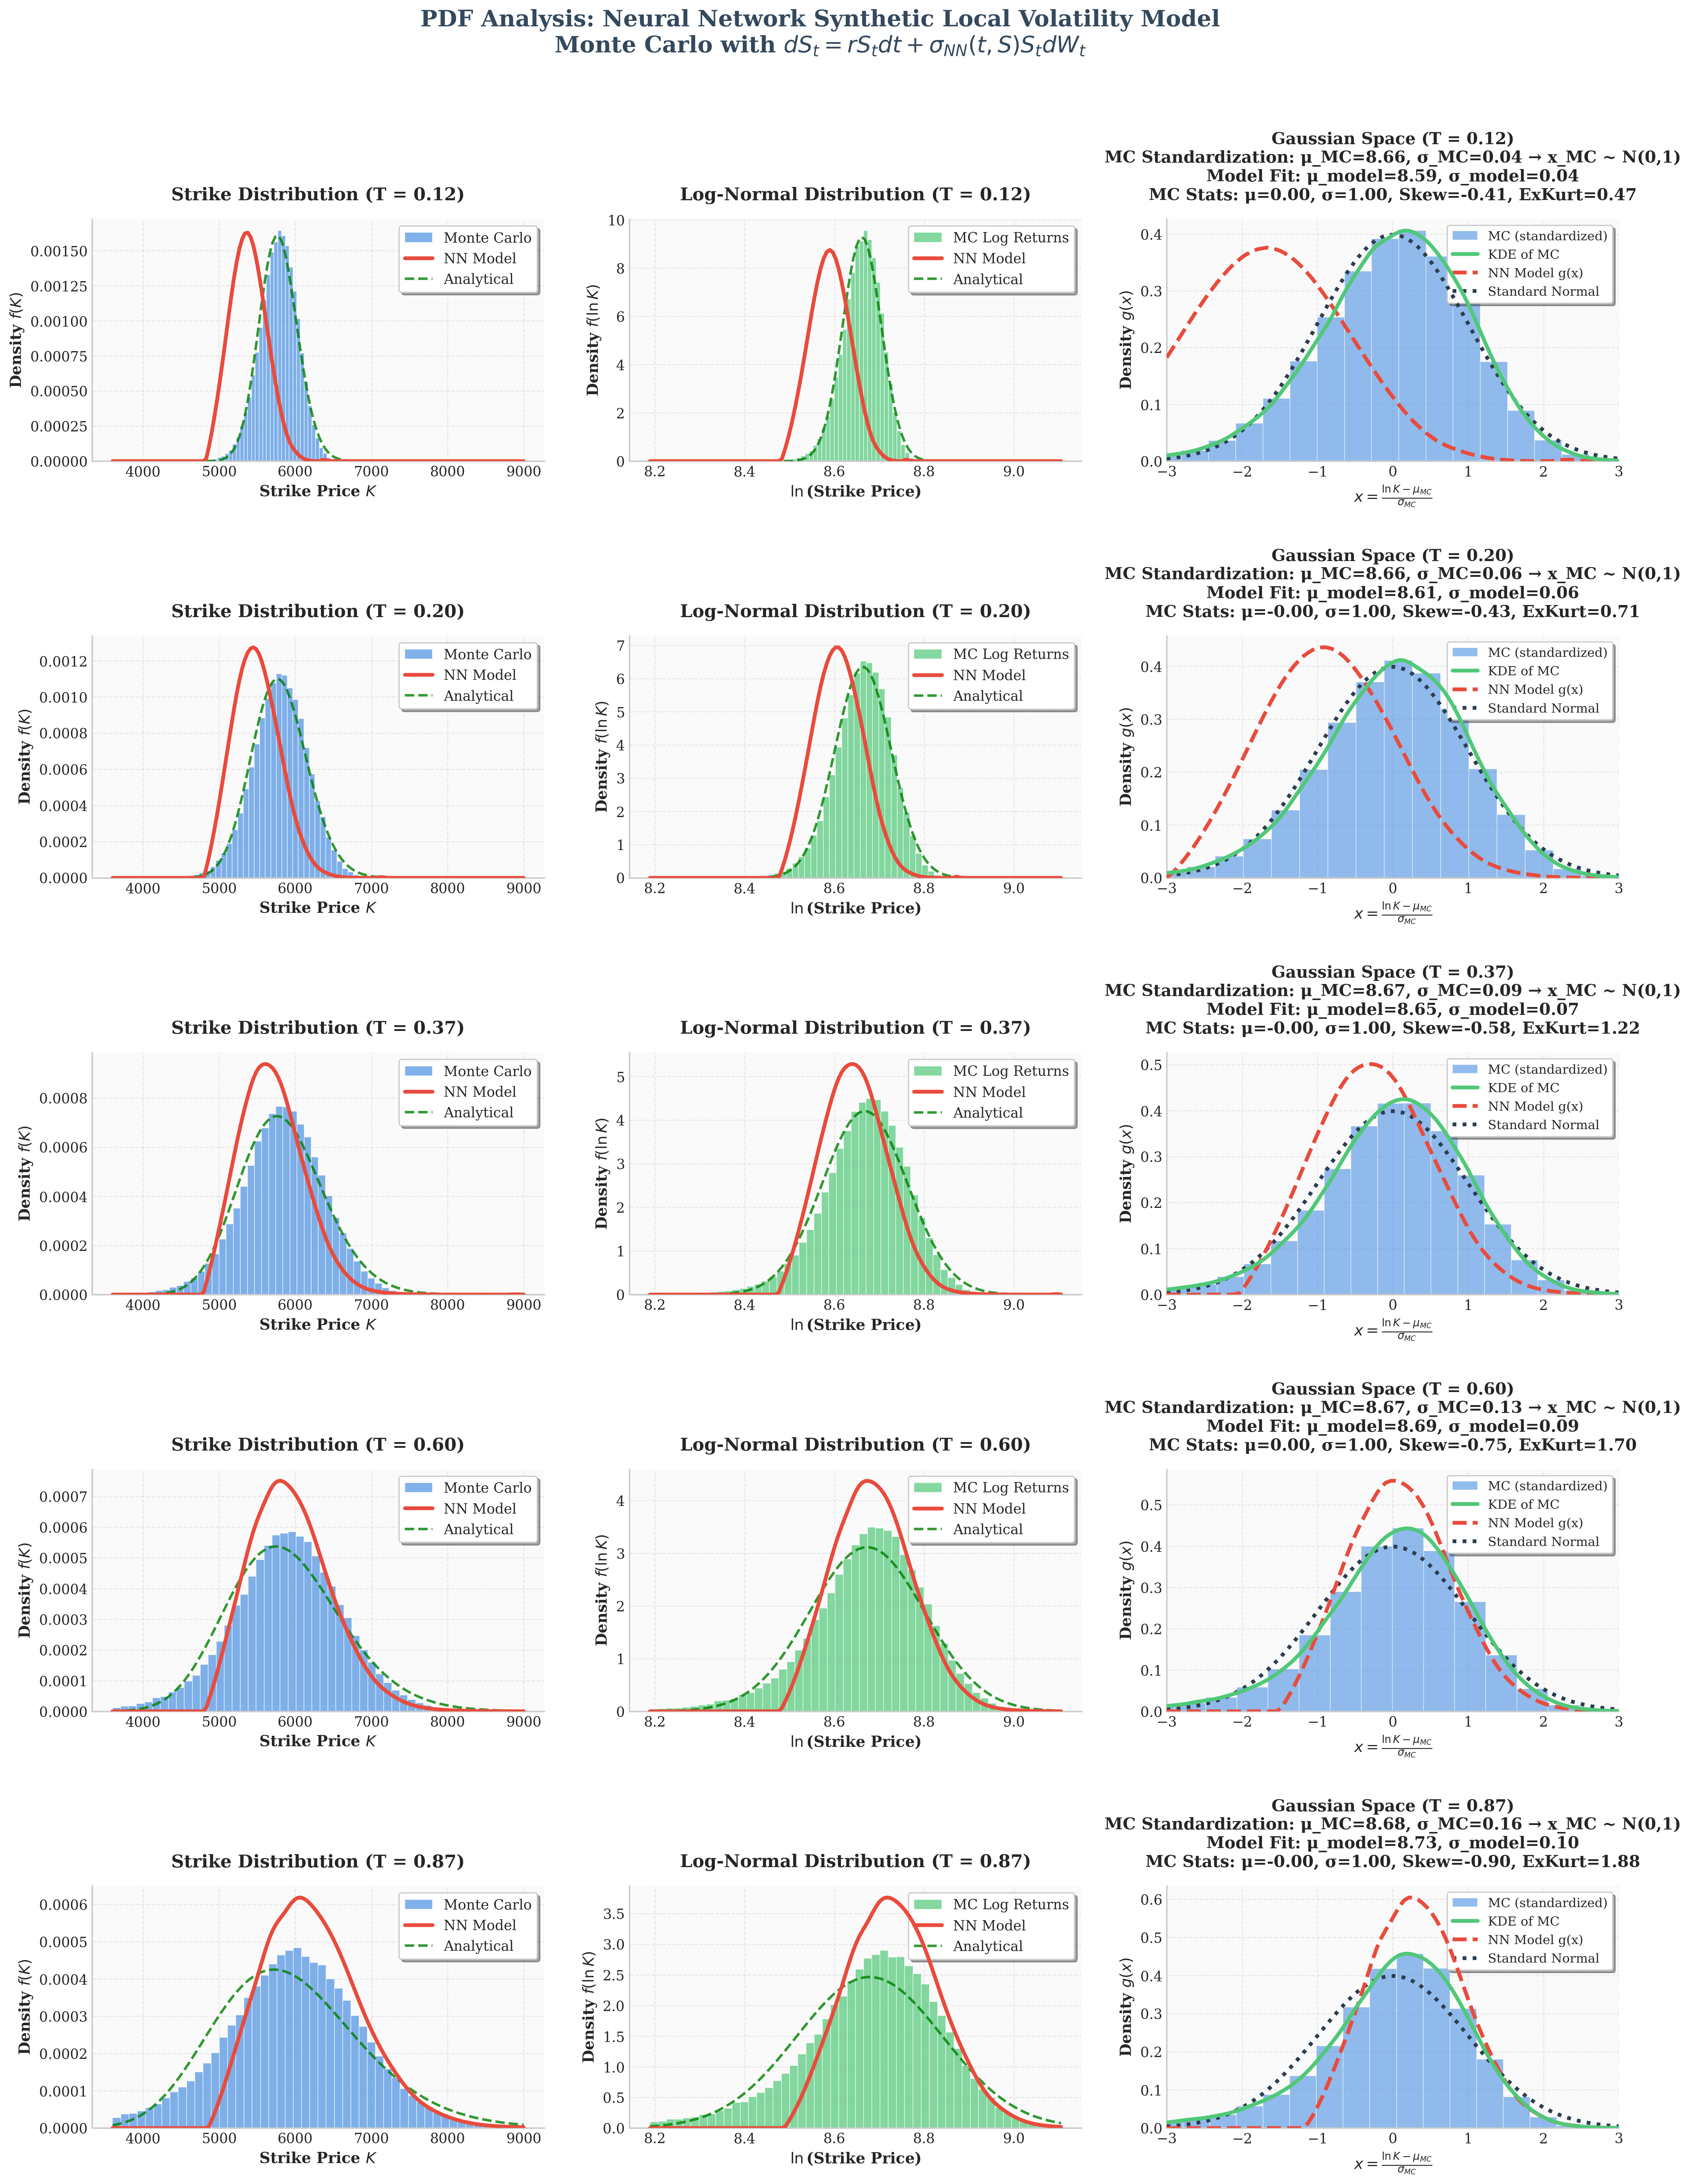
\includegraphics[width=0.92\linewidth]{figures/dec10_pdfs/dax_day2_aug8.png}
    \end{center}
    \vspace{-0.1cm}
    {\footnotesize \textbf{DAX Aug 8 2001} (provisional day assignment --- confirm via raw data).
    $K\in[4000,9000]$, $T\in\{0.12,0.20,0.37,0.60,0.87\}$; $\mu_{\mathrm{MC}}=8.66$ ($\ln K$).
    Same structural pattern as Aug 7: K-space NN deviation, Gaussian-space MC on target.}
\end{frame}

\begin{frame}{Case 3: DAX Aug 9, 2001 --- PDF analysis}
    \begin{center}
        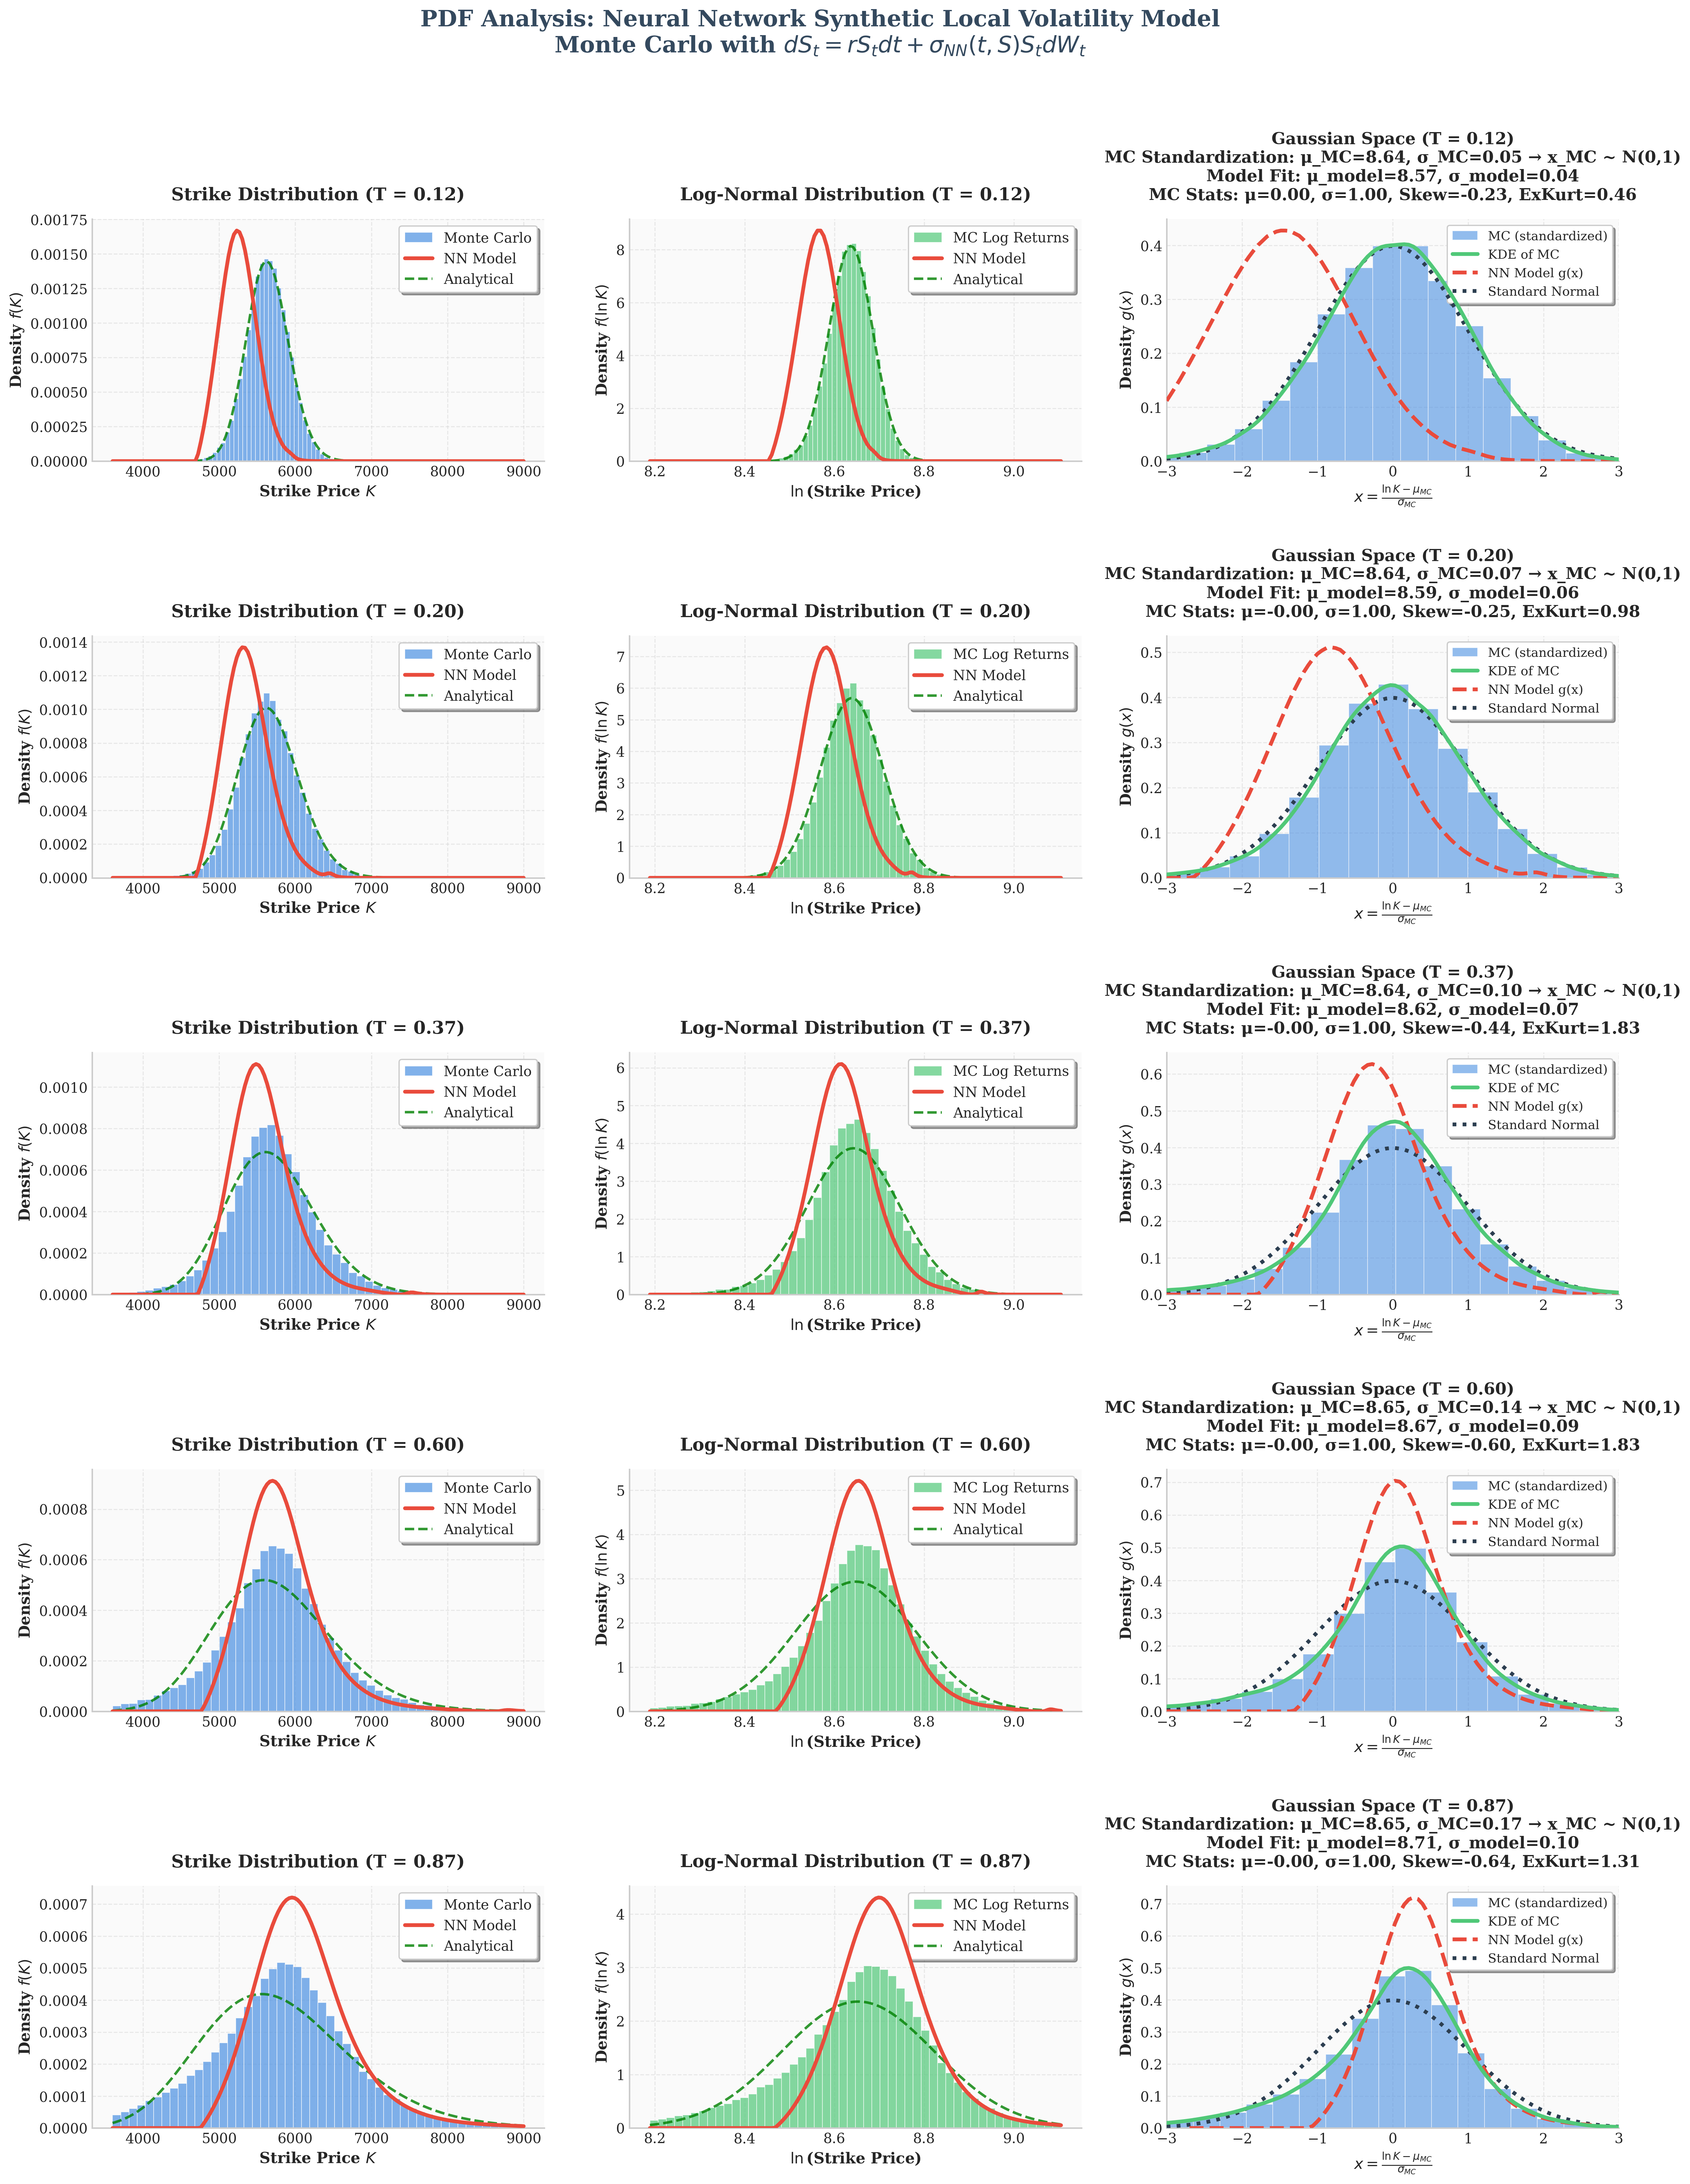
\includegraphics[width=0.92\linewidth]{figures/dec10_pdfs/dax_day3_aug9.png}
    \end{center}
    \vspace{-0.1cm}
    {\footnotesize \textbf{DAX Aug 9 2001} (provisional day assignment --- confirm via raw data).
    $K\in[4000,9000]$, $T\in\{0.12,0.20,0.37,0.60,0.87\}$; $\mu_{\mathrm{MC}}=8.64$ ($\ln K$).
    Three-day window shows consistent K=0 boundary effect across consecutive trading days.}
\end{frame}

%% ============================================================
\section{IBP three-way diagnostic}
%% ============================================================

\begin{frame}{IBP three-way diagnostic: $M_1$, $M_2$, $M_3$}
    For each maturity $T$, compute three independent estimates of $\mathbb{E}[S_T]$
    from the trained NN pair $(\mathrm{NN}_\varphi, \mathrm{NN}_\eta)$:
    \begin{align*}
        M_1 &= e^{rT}\!\int_0^\infty\!\! K\,\frac{\partial^2 C_{\mathrm{NN}}}{\partial K^2}\,dK
            && \text{(density quadrature)} \\
        M_2 &= e^{rT}\,C_{\mathrm{NN}}(0,T)
            && \text{(IBP closed form)} \\
        M_3 &= \mathbb{E}[S_T]\ \text{from MC with}\ \sigma_{\mathrm{NN}}(t,S)
            && \text{(Dupire forward simulation)}
    \end{align*}
    Under no-arbitrage all three should equal $S_0 e^{rT}$.

    \vspace{0.4em}
    \footnotesize
    \setlength{\tabcolsep}{4pt}
    \centering
    \begin{tabular}{r r r r r r r r r r}
        \toprule
        $T$ & $M_{\mathrm{ref}}$ & $M_1$ & \%err & $M_2$ & \%err & $M_3$ & \%err & $\Delta M_{12}\%$ & $\Delta M_{13}\%$ \\
        \midrule
        0.5 & 1020.20 &  948.87 & $-6.99$ &  948.93 & $-6.99$ & 1018.25 & $-0.19$ & 0.006 & 6.814 \\
        1.0 & 1040.81 &  967.66 & $-7.03$ &  967.74 & $-7.02$ & 1038.19 & $-0.25$ & 0.009 & 6.794 \\
        1.5 & 1061.84 &  982.49 & $-7.47$ &  982.95 & $-7.43$ & 1054.36 & $-0.70$ & 0.047 & 6.816 \\
        \bottomrule
    \end{tabular}

    \vspace{0.2em}
    \scriptsize
    Pretrained \texttt{models/example\_pretrained} on the manuscript Dupire surface.
\end{frame}

\begin{frame}{Discrepancy: $\Delta M_{12}$ and $\Delta M_{13}$ vs maturity}
    \begin{center}
        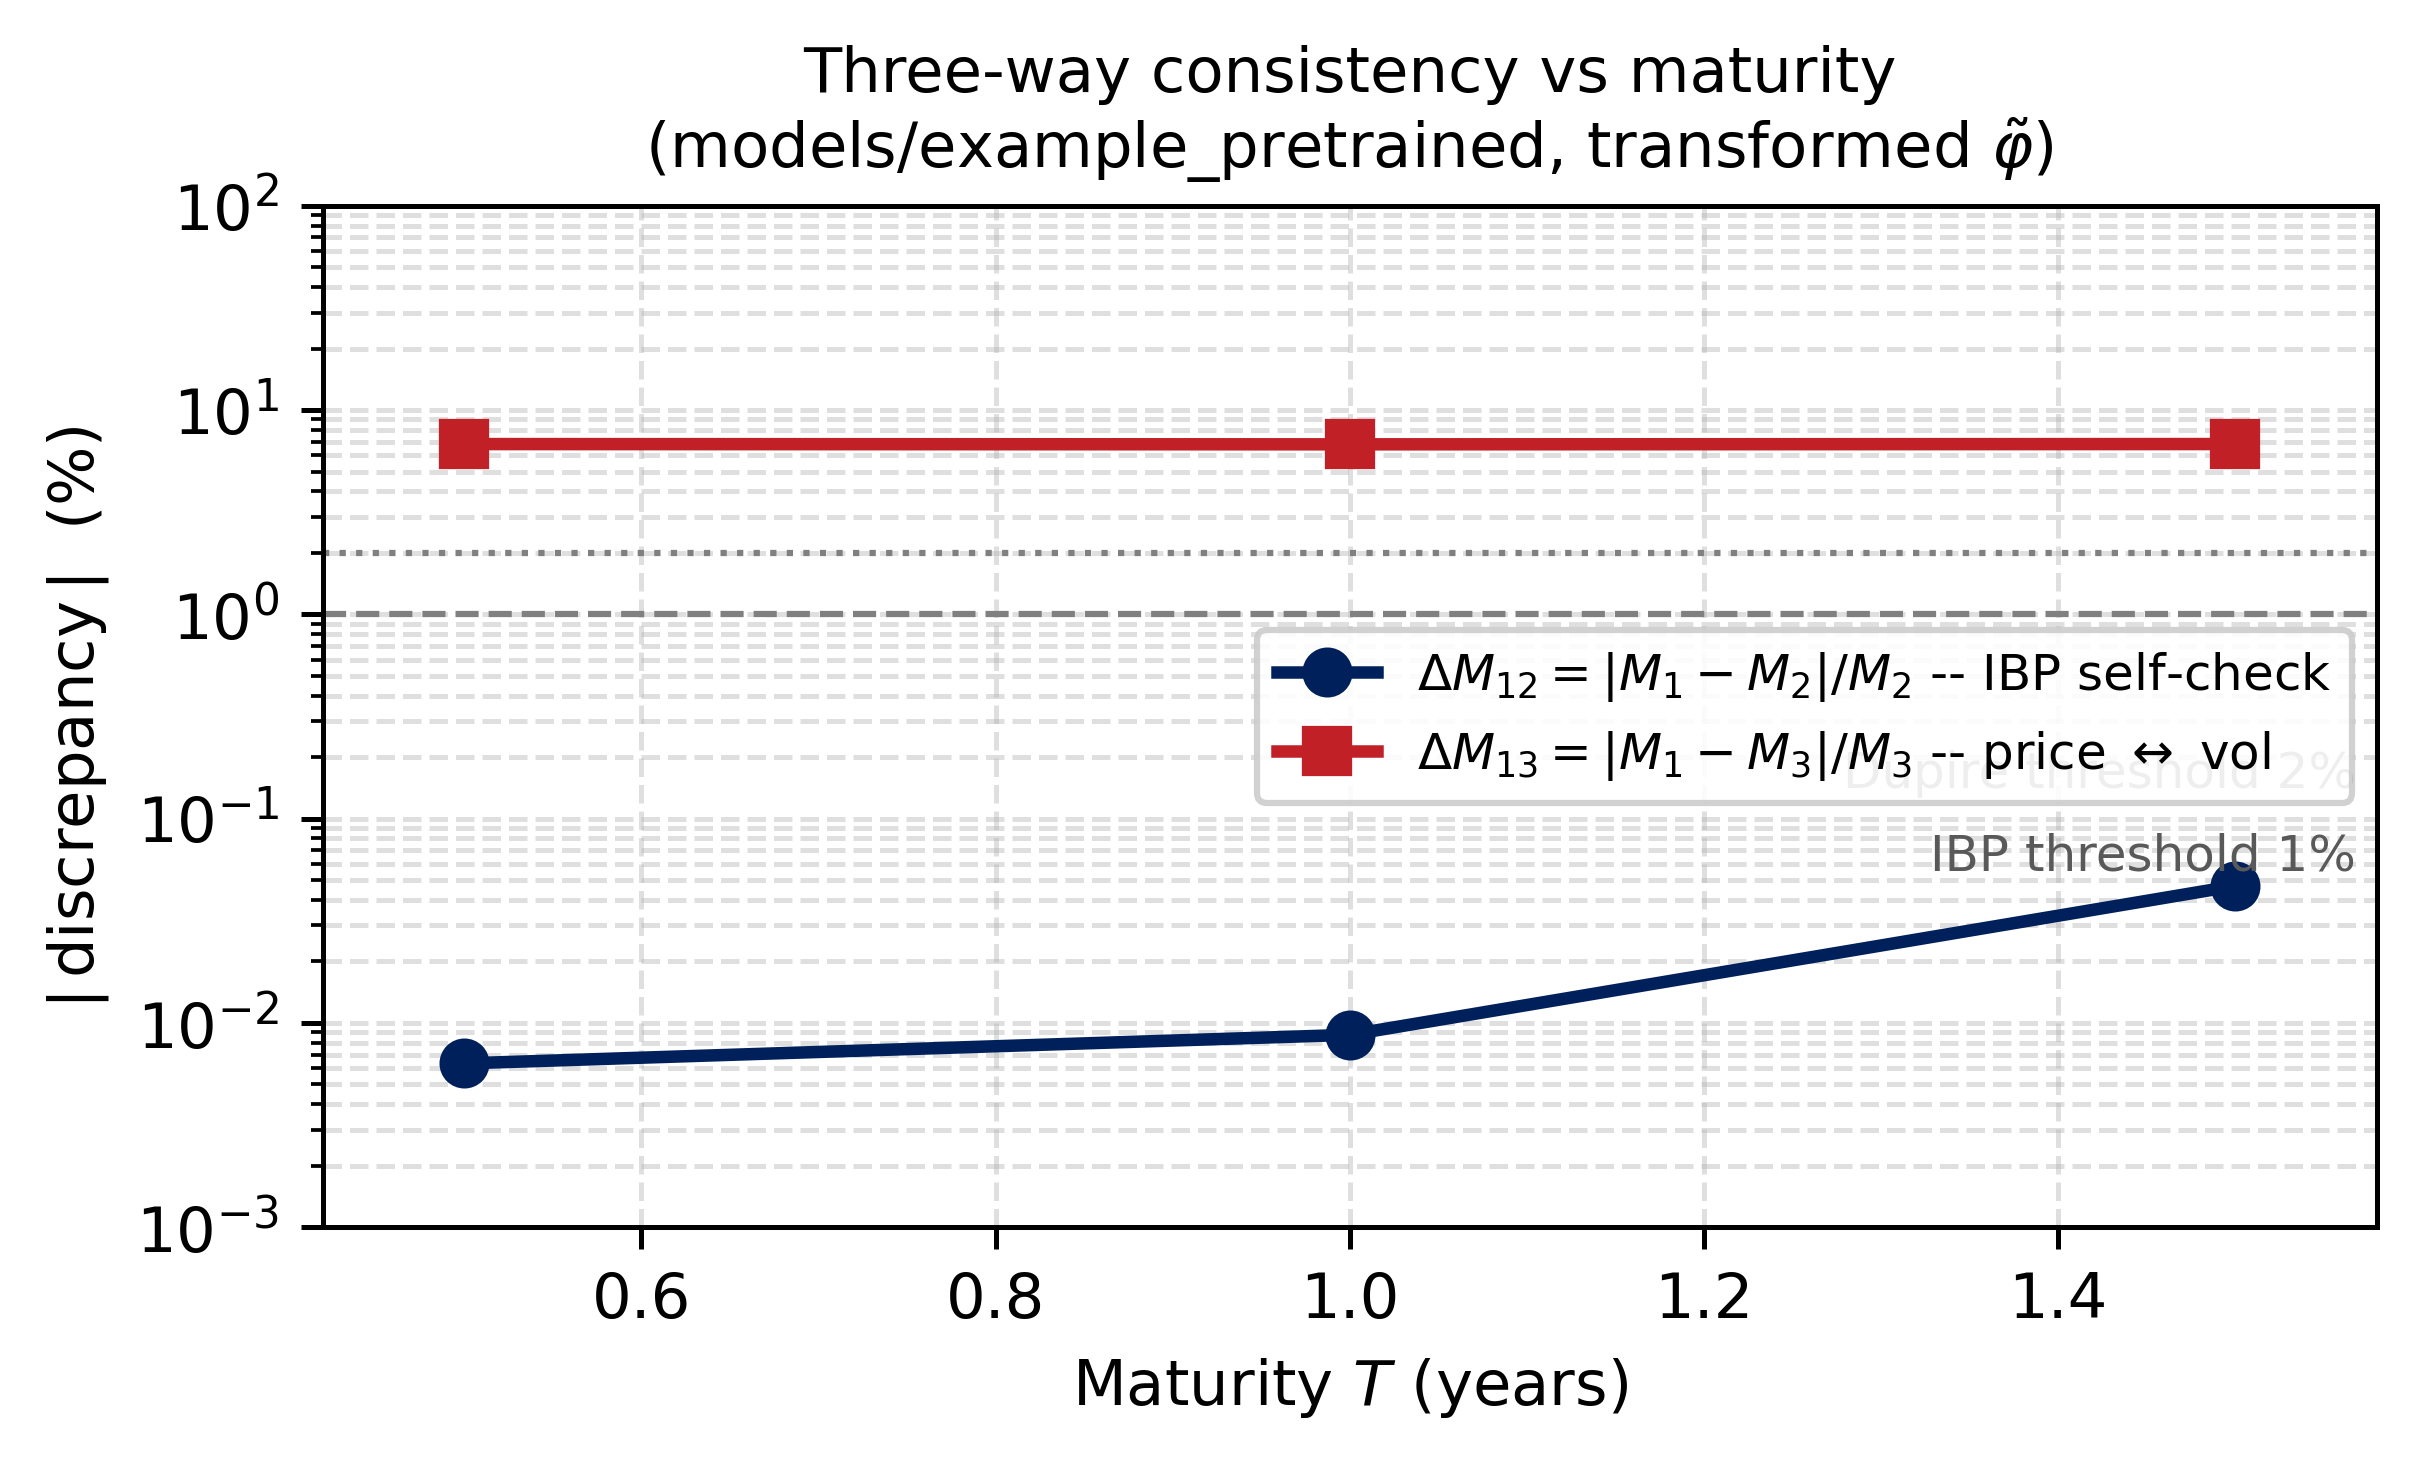
\includegraphics[width=0.78\linewidth,keepaspectratio]{ibp_deltas_vs_T.png}
    \end{center}
    \vspace{-0.3em}
    \begin{itemize}\setlength{\itemsep}{0.2em}
        \item $\Delta M_{12} \equiv |M_1-M_2|/M_2 < 0.05\%$ everywhere
              $\Rightarrow$ IBP identity holds to machine precision; autodiff and quadrature agree.
        \item $\Delta M_{13} \equiv |M_1-M_3|/M_3 \approx 6.8\%$ \textbf{at every maturity}
              $\Rightarrow$ a systematic, $T$-independent gap between the price-NN and the vol-NN legs.
        \item $M_3$ within $0.7\%$ of forward $\Rightarrow$ $\mathrm{NN}_\eta$ is well-calibrated;
              the gap lives entirely in $\mathrm{NN}_\varphi$.
    \end{itemize}
\end{frame}

\begin{frame}{Hypothesis: the $K\!=\!0$ boundary is structurally unreachable}
    \small
    \textbf{Implemented} call-price ansatz (as trained, \texttt{neural\_phi\_tilde}):
    \[
        \pi^c_\theta(k,t) = S_0\bigl(1 - e^{-\mathcal{N}_c(k,t;\theta_c)}\bigr),
        \qquad \mathcal{N}_c = \text{softplus output} > 0 .
    \]
    So $\tilde\varphi = 1-e^{-\mathcal{N}_c}$ has range $(0,1)$ --- \textbf{open at $1$}.
    \begin{itemize}\setlength{\itemsep}{0.2em}
        \item $K=\infty$ ($k=1$): BC is $\tilde\varphi=0$, i.e.\ $\mathcal{N}_c=0$
              --- \textbf{attainable}.
        \item $K=0$ ($k=0$): BC is $\tilde\varphi=1$, i.e.\ $\mathcal{N}_c\to\infty$
              --- \textbf{unattainable} by a finite output. Hence
              $C_{\mathrm{NN}}(0,T) < S_0$ by construction of the map, and the gap is our $7\%$.
    \end{itemize}
    {\footnotesize (Eq.~3.9 of the manuscript carries an extra $(1-k)$ factor that is
    \emph{not} in the code. It would not help here: at $k=0$, $(1-k)=1$, so the $K=0$
    deficit persists either way.)}
    \vspace{0.2em}

    \textbf{Why the deficit is constant in $T$:} the rescaled Dupire PDE
    $\partial_t\pi = \eta\,k^2\,\partial^2_k\pi$ carries a $k^2$ factor that vanishes
    at $k=0$, so $\pi^c_\theta(0,t)=\pi^c_\theta(0,0)$ for all $t$: the $T=0$ deficit
    is frozen across every maturity --- exactly the flat $\Delta M_{13}\!\approx\!7\%$.
\end{frame}

\begin{frame}{Direct check: evaluate $\mathcal{N}_c$ at the boundaries}
    \small
    Evaluate the trained network at $k=0$ and $k=1$ (\texttt{models/example\_pretrained}):
    \vspace{0.3em}
    \setlength{\tabcolsep}{6pt}
    \centering
    \begin{tabular}{r r r r r r}
        \toprule
        $T$ & $\mathcal{N}_c(0,T)$ & $\tilde\varphi(0,T)$ & deficit & $\mathcal{N}_c(1,T)$ & $\tilde\varphi(1,T)$ \\
        \midrule
        0.5 & 2.661 & 0.9301 & $6.99\%$ & 0.0007 & 0.0007 \\
        1.0 & 2.656 & 0.9298 & $7.02\%$ & 0.0128 & 0.0128 \\
        1.5 & 2.600 & 0.9257 & $7.43\%$ & 0.0315 & 0.0310 \\
        \bottomrule
    \end{tabular}

    \vspace{0.2em}
    {\footnotesize $\mathcal{N}_c(0,T)\!\approx\!2.6$ (finite --- would need $\infty$) vs.\
    $\mathcal{N}_c(1,T)\!\approx\!0.01$: two orders of magnitude. The far boundary is nearly
    reached; $K\!=\!0$ is not. $e^{rT}C_{\mathrm{NN}}(0,T)$ reproduces $M_2 = 948.9 / 967.7 / 983.0$.}

    \begin{center}
        
\includegraphics[width=0.97\linewidth,height=0.42\textheight,keepaspectratio]{nn_at_k0.png}
    \end{center}
\end{frame}

%% ============================================================
\section{Summary}
%% ============================================================

\begin{frame}{Summary}
    \begin{itemize}\setlength{\itemsep}{0.3em}
        \item Across constant-$\sigma$, manuscript Dupire, and DAX market data,
              the published NN pair fits the in-window grid well.
        \item The IBP three-way test reveals a $T$-independent $\sim\!7\%$ gap
              between $M_1\!=\!M_2$ and $M_3$.
        \item $\Delta M_{12}$ is at machine precision; $M_3$ within $0.7\%$ of forward.
              The gap is entirely in $\mathrm{NN}_\varphi$, not $\mathrm{NN}_\eta$.
        \item Root cause: the output map $\tilde\varphi=1-e^{-\mathcal{N}_c}$ has range $(0,1)$.
              The $K\!=\!\infty$ BC ($\tilde\varphi\!=\!0$) is reachable ($\mathcal{N}_c\!=\!0$);
              the $K\!=\!0$ BC ($\tilde\varphi\!=\!1$) needs $\mathcal{N}_c\!\to\!\infty$ and is not.
              The Dupire PDE degenerates at $k\!=\!0$, freezing the deficit across $T$.
              Confirmed directly: $\mathcal{N}_c(0,T)\!\approx\!2.6$, $\mathcal{N}_c(1,T)\!\approx\!0.01$.
    \end{itemize}
\end{frame}

\end{document}
